%%%%%%%%%%%%%%%%%%%%%%%%%%%%%%%%%%%%%%%%%%%%%%%%%%%%%%%%%%%%%%%
% Document Class and Basic Settings
%%%%%%%%%%%%%%%%%%%%%%%%%%%%%%%%%%%%%%%%%%%%%%%%%%%%%%%%%%%%%%%
\documentclass[12pt, a4paper]{report}

% Encoding and Language
\usepackage[T1]{fontenc}
\usepackage[latin1]{inputenc}
\usepackage[english]{babel}
\usepackage{xcolor}
\usepackage{tcolorbox}
\usepackage{tikz}
\usepackage{pgf-umlsd} 
\usepackage{dirtree}

%%%%%%%%%%%%%%%%%%%%%%%%%%%%%%%%%%%%%%%%%%%%%%%%%%%%%%%%%%%%%%%
% Page Layout and Geometry
%%%%%%%%%%%%%%%%%%%%%%%%%%%%%%%%%%%%%%%%%%%%%%%%%%%%%%%%%%%%%%%
\usepackage[
  left=1.4in,
  right=1.4in,
  top=0.5in,
  bottom=0.5in,
  headheight=26pt,
  includeheadfoot
]{geometry}


%%%%%%%%%%%%%%%%%%%%%%%%%%%%%%%%%%%%%%%%%%%%%%%%%%%%%%%%%%%%%%%
% Mathematics, Graphics, and Tables
%%%%%%%%%%%%%%%%%%%%%%%%%%%%%%%%%%%%%%%%%%%%%%%%%%%%%%%%%%%%%%%
\usepackage{amsmath}
\usepackage{graphicx}
\usepackage{booktabs}       % High-quality tables
\usepackage{multirow}
\usepackage{lscape}
\usepackage{caption}
\usepackage[flushleft]{threeparttable}
\usepackage{tikz}
\usepackage{pgf-umlsd}


%%%%%%%%%%%%%%%%%%%%%%%%%%%%%%%%%%%%%%%%%%%%%%%%%%%%%%%%%%%%%%%
% Code Listings and MATLAB Prettifier
%%%%%%%%%%%%%%%%%%%%%%%%%%%%%%%%%%%%%%%%%%%%%%%%%%%%%%%%%%%%%%%
\usepackage{listings}
\usepackage[framed,numbered]{matlab-prettifier}
\usepackage{minted}


%%%%%%%%%%%%%%%%%%%%%%%%%%%%%%%%%%%%%%%%%%%%%%%%%%%%%%%%%%%%%%%
% Hyperlinks, Dates, and Colors
%%%%%%%%%%%%%%%%%%%%%%%%%%%%%%%%%%%%%%%%%%%%%%%%%%%%%%%%%%%%%%%
%%%%%%%%%%%%%%%%%%%%%%%%%%%%%%%%%%%%%%%%%%%%%%%%%%%%%%%%%%%%%%%
% Hyperlinks, Dates, and Colors
%%%%%%%%%%%%%%%%%%%%%%%%%%%%%%%%%%%%%%%%%%%%%%%%%%%%%%%%%%%%%%%
\usepackage{xcolor}
\definecolor{blue1}{RGB}{0,73,114}
\definecolor{blue2}{RGB}{89,128,183}

\usepackage{sectsty} % provides \chapterfont, \sectionfont, etc.
\chapterfont{\color{blue1}}    % sets chapter titles to blue1
\sectionfont{\color{blue2}}    % sets section titles to blue2
\subsectionfont{\color{blue2}}
\subsubsectionfont{\color{blue2}}

\usepackage{hyperref} % load hyperref without extra color options
% Load hyperref with specific settings
\hypersetup{
    colorlinks=true,       % true: colored links instead of boxes
    linkcolor=black,       % color of internal links in ToC (same as text color for invisibility)
    citecolor=red,         % color of citation links
    filecolor=magenta,     % color of file links
    urlcolor=black,         % color of external links
    linktoc=all,           % 'all' will create links for everything in toc
    pdfborderstyle={/S/U/W 0} % no visible borders
}

% Customize Table of Contents, List of Figures, and List of Tables titles
\usepackage{tocloft}

% Style for "Contents" title
\renewcommand{\cfttoctitlefont}{\huge\bfseries\color{blue1}}

% Style for "List of Figures" title
\renewcommand{\cftloftitlefont}{\huge\bfseries\color{blue1}}

% Style for "List of Tables" title
\renewcommand{\cftlottitlefont}{\huge\bfseries\color{blue1}}

% If you're not using the tocloft package already, an alternative approach is:
\makeatletter
\renewcommand\tableofcontents{%
    \section*{\textcolor{blue1}{\contentsname}}%
    \@starttoc{toc}%
}
\renewcommand\listoffigures{%
    \section*{\textcolor{blue1}{\listfigurename}}%
    \@starttoc{lof}%
}
\renewcommand\listoftables{%
    \section*{\textcolor{blue1}{\listtablename}}%
    \@starttoc{lot}%
}
\makeatother

%%%%%%%%%%%%%%%%%%%%%%%%%%%%%%%%%%%%%%%%%%%%%%%%%%%%%%%%%%%%%%%
% Additional Formatting Packages
%%%%%%%%%%%%%%%%%%%%%%%%%%%%%%%%%%%%%%%%%%%%%%%%%%%%%%%%%%%%%%%
\usepackage{titlesec}       % Custom section spacing
\usepackage{titling}        % Custom title formatting
\usepackage{fancyhdr}       % Headers and footers
\usepackage{tocloft}        % Table of contents formatting
\usepackage{setspace}       % Line spacing
\usepackage{enumitem}       % Customized lists
\usepackage{indentfirst}    % Indent first paragraph of sections
\usepackage{float}          % Improved float control
\usepackage{comment}        % For commenting out blocks of text
\usepackage{nomencl}        % For nomenclature (if needed)
\usepackage{lipsum}         % Dummy text (for testing)


%%%%%%%%%%%%%%%%%%%%%%%%%%%%%%%%%%%%%%%%%%%%%%%%%%%%%%%%%%%%%%%
% Enhanced Spacing Settings
%%%%%%%%%%%%%%%%%%%%%%%%%%%%%%%%%%%%%%%%%%%%%%%%%%%%%%%%%%%%%%%
\usepackage{parskip} % Better paragraph spacing
\setlength{\parskip}{1.5ex plus 0.5ex minus 0.2ex}  % Space between paragraphs
\setlength{\parsep}{0.5ex plus 0.2ex minus 0.1ex}    % Space within paragraphs
\setlength{\itemsep}{1ex plus 0.5ex minus 0.2ex}     % Space between list items
\setlength{\topsep}{2ex plus 0.5ex minus 0.2ex}       % Space above/below lists
\setlength{\partopsep}{1ex plus 0.5ex minus 0.2ex}    % Extra space around lists

%%%%%%%%%%%%%%%%%%%%%%%%%%%%%%%%%%%%%%%%%%%%%%%%%%%%%%%%%%%%%%%
% Section Spacing Customization
%%%%%%%%%%%%%%%%%%%%%%%%%%%%%%%%%%%%%%%%%%%%%%%%%%%%%%%%%%%%%%%
\titlespacing*{\section}{0pt}{3.5ex plus 1ex minus .2ex}{2.3ex plus .2ex}
\titlespacing*{\subsection}{0pt}{3.25ex plus 1ex minus .2ex}{1.5ex plus .2ex}

%%%%%%%%%%%%%%%%%%%%%%%%%%%%%%%%%%%%%%%%%%%%%%%%%%%%%%%%%%%%%%%
% Listings Settings (MATLAB)
%%%%%%%%%%%%%%%%%%%%%%%%%%%%%%%%%%%%%%%%%%%%%%%%%%%%%%%%%%%%%%%
\lstset{
  language=Matlab,
  style=Matlab-editor,
  basicstyle=\normalsize\mlttfamily,
  numbers=left,
  numberstyle=\scriptsize\color{black},
  numbersep=0.5cm,
  lineskip=2pt  % Space between lines in listings
}

% Custom Enumerate Environment for Steps
\newlist{steps}{enumerate}{1}
\setlist[steps,1]{leftmargin=1.5cm, label=Step \arabic*:, itemsep=1ex}

%%%%%%%%%%%%%%%%%%%%%%%%%%%%%%%%%%%%%%%%%%%%%%%%%%%%%%%%%%%%%%%
% Header & Footer Configuration
%%%%%%%%%%%%%%%%%%%%%%%%%%%%%%%%%%%%%%%%%%%%%%%%%%%%%%%%%%%%%%%
% \pagestyle{fancy}
% \fancyhf{}  % Clear default header/footer

% Header: Use the document title
\lhead{\thetitle}
\setlength{\headheight}{16pt}

% Footer: Display page number and reference to the last main page
\cfoot{Page \thepage\ of \pageref{endOfDoc}}
\renewcommand{\headrulewidth}{1pt}
\renewcommand{\footrulewidth}{1pt}

%%%%%%%%%%%%%%%%%%%%%%%%%%%%%%%%%%%%%%%%%%%%%%%%%%%%%%%%%%%%%%%
% Font Settings
%%%%%%%%%%%%%%%%%%%%%%%%%%%%%%%%%%%%%%%%%%%%%%%%%%%%%%%%%%%%%%%

\renewcommand{\rmdefault}{ptm}

%%%%%%%%%%%%%%%%%%%%%%%%%%%%%%%%%%%%%%%%%%%%%%%%%%%%%%%%%%%%%%%
% Title and Document Information
%%%%%%%%%%%%%%%%%%%%%%%%%%%%%%%%%%%%%%%%%%%%%%%%%%%%%%%%%%%%%%%
\title{The Blockchain Transaction Information Visualization System}
\makeatletter
\let\Title\@title
\makeatother

%%%%%%%%%%%%%%%%%%%%%%%%%%%%%%%%%%%%%%%%%%%%%%%%%%%%%%%%%%%%%%%
% Begin Document
%%%%%%%%%%%%%%%%%%%%%%%%%%%%%%%%%%%%%%%%%%%%%%%%%%%%%%%%%%%%%%%
\begin{document}

%-------------------------------
% Front Page
%-------------------------------
\begin{titlepage}
\begin{center}
    \textsc{\Large \bfseries Swinburne University of Technology}\\[0.3cm]
    \textsc{\large Ho Chi Minh Campus}\\
    \textsc{\large Semester 1, 2025}
    
    
\includegraphics[width=0.7\textwidth]{root/swinburne-university-of-technology-7-logo-png-transparent.png}
    
    % Title
    \hrule
    \vspace{.2cm}
    {\huge\bfseries The Blockchain Transaction\\\vspace{0.5cm} Information Visualization System} % title of the report
    \vspace{.2cm}
    \hrule

    \vspace{0.5cm}
    
    \textsc{\large\textbf{Authors}}\\
    \vspace{.5cm}
    \centering
    % authors
    Ky Anh Nguyen - 105103551\\
    Pham Thanh Truc Tran - 104813707\\
    Pham Hanh Nguyen Dinh - 105532896\\
    Quoc Anh Nguyen - 104849210\\[1cm]
      \textsc{\large\textbf{Github Link}}\\
    \vspace{.3cm}
    \centering
    \href{https://github.com/orgs/SwinHCMC-COS30049/repositories}{COS30049 Repositories}\\ 
     \vspace{.3cm}
    \textsc{\large\textbf{Instructor}}\\
    \vspace{.3cm}
    Tristan Nguyen\\[0.5cm]
    \centering \today % see latexmkrc for time zone change
\end{center}
\end{titlepage}
\newpage

%-------------------------------
% Table of Contents (not counted in page numbering)
%-------------------------------
\tableofcontents

%-------------------------------
% Lists (Figures and Tables)
%-------------------------------
% \pagenumbering{arabic}
% Setup for JSON code listings
\definecolor{codegray}{rgb}{0.95,0.95,0.95}
\definecolor{codegreen}{rgb}{0.0,0.6,0.0}
\definecolor{codepurple}{rgb}{0.58,0,0.82}
\definecolor{backcolour}{rgb}{0.95,0.95,0.95}


\lstdefinestyle{json}{
    backgroundcolor=\color{backcolour},   
    commentstyle=\color{codegreen},
    keywordstyle=\color{codepurple},
    stringstyle=\color{codegreen},
    breaklines=true,
    breakatwhitespace=true,
    tabsize=2,
    basicstyle=\ttfamily\small,
    frame=single
}


\newpage
\phantomsection
\addcontentsline{toc}{section}{List of Figures}
\listoffigures

\newpage
\phantomsection
\addcontentsline{toc}{section}{List of Tables}
\listoftables

\newpage

%-------------------------------
% Main Content
%-------------------------------
\section*{Team Introduction} \label{ch2}
Our project team consists of four full-stack developers, each contributing to both frontend and backend development while maintaining specific leadership responsibilities:

\begin{itemize}
    \item \textbf{Team Lead}
    \begin{itemize}
        \item \textbf{Ky Anh Nguyen} - Full Stack Developer, Project Lead
        \begin{itemize}
            \item Led overall project direction and technical architecture
            \item Coordinated team activities and milestone delivery
            \item Contributed to both frontend and backend development
        \end{itemize}
    \end{itemize}
    
    \item \textbf{Team Members}
    \begin{itemize}
        \item \textbf{Pham Thanh Truc Tran} - Full Stack Developer
        \begin{itemize}
            \item Specialized in frontend development while maintaining full-stack capabilities
            \item Contributed to system architecture and implementation
        \end{itemize}
        \item \textbf{Pham Hanh Nguyen Dinh} - Quality Assurance 
        \begin{itemize}
            \item Data Validation Testing
            \item User Interface Testing
            \item Performance Testing            
        \end{itemize}
        \item \textbf{Quoc Anh Nguyen} - Full Stack Developer
        \begin{itemize}
            \item Contributed to both frontend and backend development
            \item Participated in system design and implementation
        \end{itemize}
    \end{itemize}
\end{itemize}

As a team of full-stack developers, we maintained a flexible and collaborative approach throughout the project lifecycle. Each member contributed across the entire technology stack, allowing for efficient resource allocation and comprehensive problem-solving. This versatility enabled us to adapt quickly to challenges and ensure consistent progress across all aspects of the project.
\newpage

\chapter{Introduction} \label{ch1}

\section{Background}
Over the past decade, "Blockchain" has become a ubiquitous term across media, popular discourse, and academic literature, particularly following Satoshi Nakamoto's introduction of Bitcoin cryptocurrency in 2008 \cite{wright2008bitcoin}. Despite its widespread recognition, blockchain remains a relatively nascent technology whose practical applications continue to evolve and are often misunderstood. A common misconception equates blockchain with Bitcoin, when in fact, blockchain technology serves as the fundamental infrastructure that enables Bitcoin and numerous other applications.

At its core, blockchain functions as a distributed digital record-keeping system that ensures transactions cannot be secretly altered or tampered with. Unlike traditional systems that rely on central authorities like banks or governments, blockchains operate through a network of users who collectively maintain and verify the shared ledger. The technology works by grouping cryptographically signed transactions into blocks, with each new block linking to its predecessor through sophisticated cryptographic methods. This creates an increasingly secure chain where older records become progressively harder to alter, while multiple copies of the ledger exist throughout the network with built-in protocols that automatically resolve any discrepancies \cite{yaga2018blockchain}.

\section{Context}
Blockchain technology, as implemented in Bitcoin, facilitates peer-to-peer transactions characterized by decentralization, cryptographic security, and transparency. This distributed ledger system enables various financial operations, including e-commerce transactions, digital asset custody, and value transfer, without traditional intermediary institutions. The technology presents significant advantages in the business domain, particularly in terms of operational transparency, cryptographic security protocols, enhanced auditability, and optimized transaction efficiency with reduced costs. While these inherent benefits have attracted substantial global investment in Bitcoin and alternative cryptocurrencies, the technological complexity presents a significant barrier to comprehensive user understanding. Despite the inherent transparency of blockchain networks and their public transaction records, the technical sophistication of the data architecture poses considerable challenges for interpretation. Consequently, there exists a critical imperative for the development of sophisticated visualization tools that can facilitate intuitive analysis of transaction patterns, network metrics, and smart contract interactions, thereby democratizing access to blockchain data analytics.

\chapter{Project Requirement List and Description} \label{ch3}
\section{Project Overview}
The Blockchain Transaction Information Visualization System is a web-based platform designed to transform complex blockchain transaction data into intuitive, interactive visualizations. At its core, the system allows users to input wallet addresses and explore transaction relationships through an interactive directed graph, where nodes represent wallets and edges represent transactions between them. The platform combines frontend visualization capabilities with backend graph database architecture to provide real-time exploration of transaction networks. Users can navigate through transaction paths by clicking nodes to explore next/previous hops, while accessing detailed transaction information in tabular format. The system's primary value proposition is making blockchain transaction patterns and relationships easily discoverable and understandable for both technical and non-technical users. The project objectives are further described in Table \ref{tab:objectives}.

\section{Core Functionalities}
The Blockchain Transaction Information Visualization System is built around five essential functionalities that work together to provide users with a comprehensive blockchain data exploration experience. At its core, the system enables users to search and analyze wallet addresses through an intuitive interface, visualize transaction relationships through interactive graphs, explore connected addresses dynamically, access detailed transaction information, and leverage efficient data storage through a graph database. 

\subsection{Wallet Address Search and Information Retrieval}
\begin{itemize}
    \item Implementation of a search interface that accepts wallet addresses
    \item Display of fundamental wallet information    
\end{itemize}

\begin{table}[htbp]
\centering
\renewcommand{\arraystretch}{1.3}
\setlength{\tabcolsep}{10pt}
\begin{threeparttable}
\caption{Project Objectives}
\label{tab:objectives}
\begin{tabular}{p{0.25\textwidth}p{0.65\textwidth}}
\toprule
\textbf{Category} & \textbf{Objective} \\
\midrule
User Interface & Create an accessible and intuitive interface for blockchain transaction information exploration with interactive graph navigation capabilities for connected addresses. \\
\addlinespace
User Experience & Implement graph database organization to facilitate rapid searches, intuitive data exploration, and enhanced visual representations of financial relationships and patterns. \\
\addlinespace
Visualization & Develop interactive visualization mechanisms for transaction networks in both graph-based and tabular representations. \\
\addlinespace
Data Exploration \& Analysis & Provide comprehensive transaction information and enable efficient analysis of blockchain transaction patterns and network behaviors. \\
\bottomrule
\end{tabular}
\begin{tablenotes}[flushleft]
\small
\item Note: These objectives guide the development of the Blockchain Transaction Information Visualization System.
\end{tablenotes}
\end{threeparttable}
\end{table}

\subsection{Transaction Graph Visualization}
\begin{itemize}
    \item Development of an interactive directed graph visualization where:
    \begin{itemize}
        \item Nodes represent individual wallet addresses
        \item Edges indicate transactions between addresses
        \item Edge directionality shows the flow of transactions
        \item Visual attributes (size, color) represent transaction volumes or frequency
    \end{itemize}
\end{itemize}

\subsection{Interactive Exploration}
\begin{itemize}
    \item Implementation of node interaction features:
    \begin{itemize}
        \item Click functionality to explore connected addresses
        \item Navigation through transaction paths (next/previous hops)
        \item Zoom and pan capabilities for graph exploration
        \item Filtering options for transaction types and time periods
    \end{itemize}
\end{itemize}

\subsection{Transaction Information Display}
\begin{itemize}
    \item Creation of a detailed transaction information panel:
    \begin{itemize}
        \item Tabular format for transaction details
        \item Sorting and filtering capabilities
        \item Time-stamped transaction history
        \item Transaction status indicators
    \end{itemize}
\end{itemize}

\subsection{Graph Database Integration}
\begin{itemize}
    \item Implementation of a graph database system:
    \begin{itemize}
        \item Efficient data storage and retrieval mechanisms
        \item Optimized query performance for large transaction sets
        \item Real-time data updates and synchronization
        \item Robust data integrity measures
    \end{itemize}
\end{itemize}
These functionalities are designed to work seamlessly together, creating a fluid user experience where users can easily move from searching a wallet address to exploring its transaction network, and diving deep into specific transaction details.


\chapter{Front-end Prototype} \label{ch4}
The frontend design of the Blockchain Transaction Information Visualization System emphasizes user-centric interaction and information clarity through a thoughtfully structured interface. The design approach balances sophisticated functionality with intuitive user experience, making complex blockchain data accessible to users of varying technical backgrounds. 
\begin{figure}[h]
    \centering
    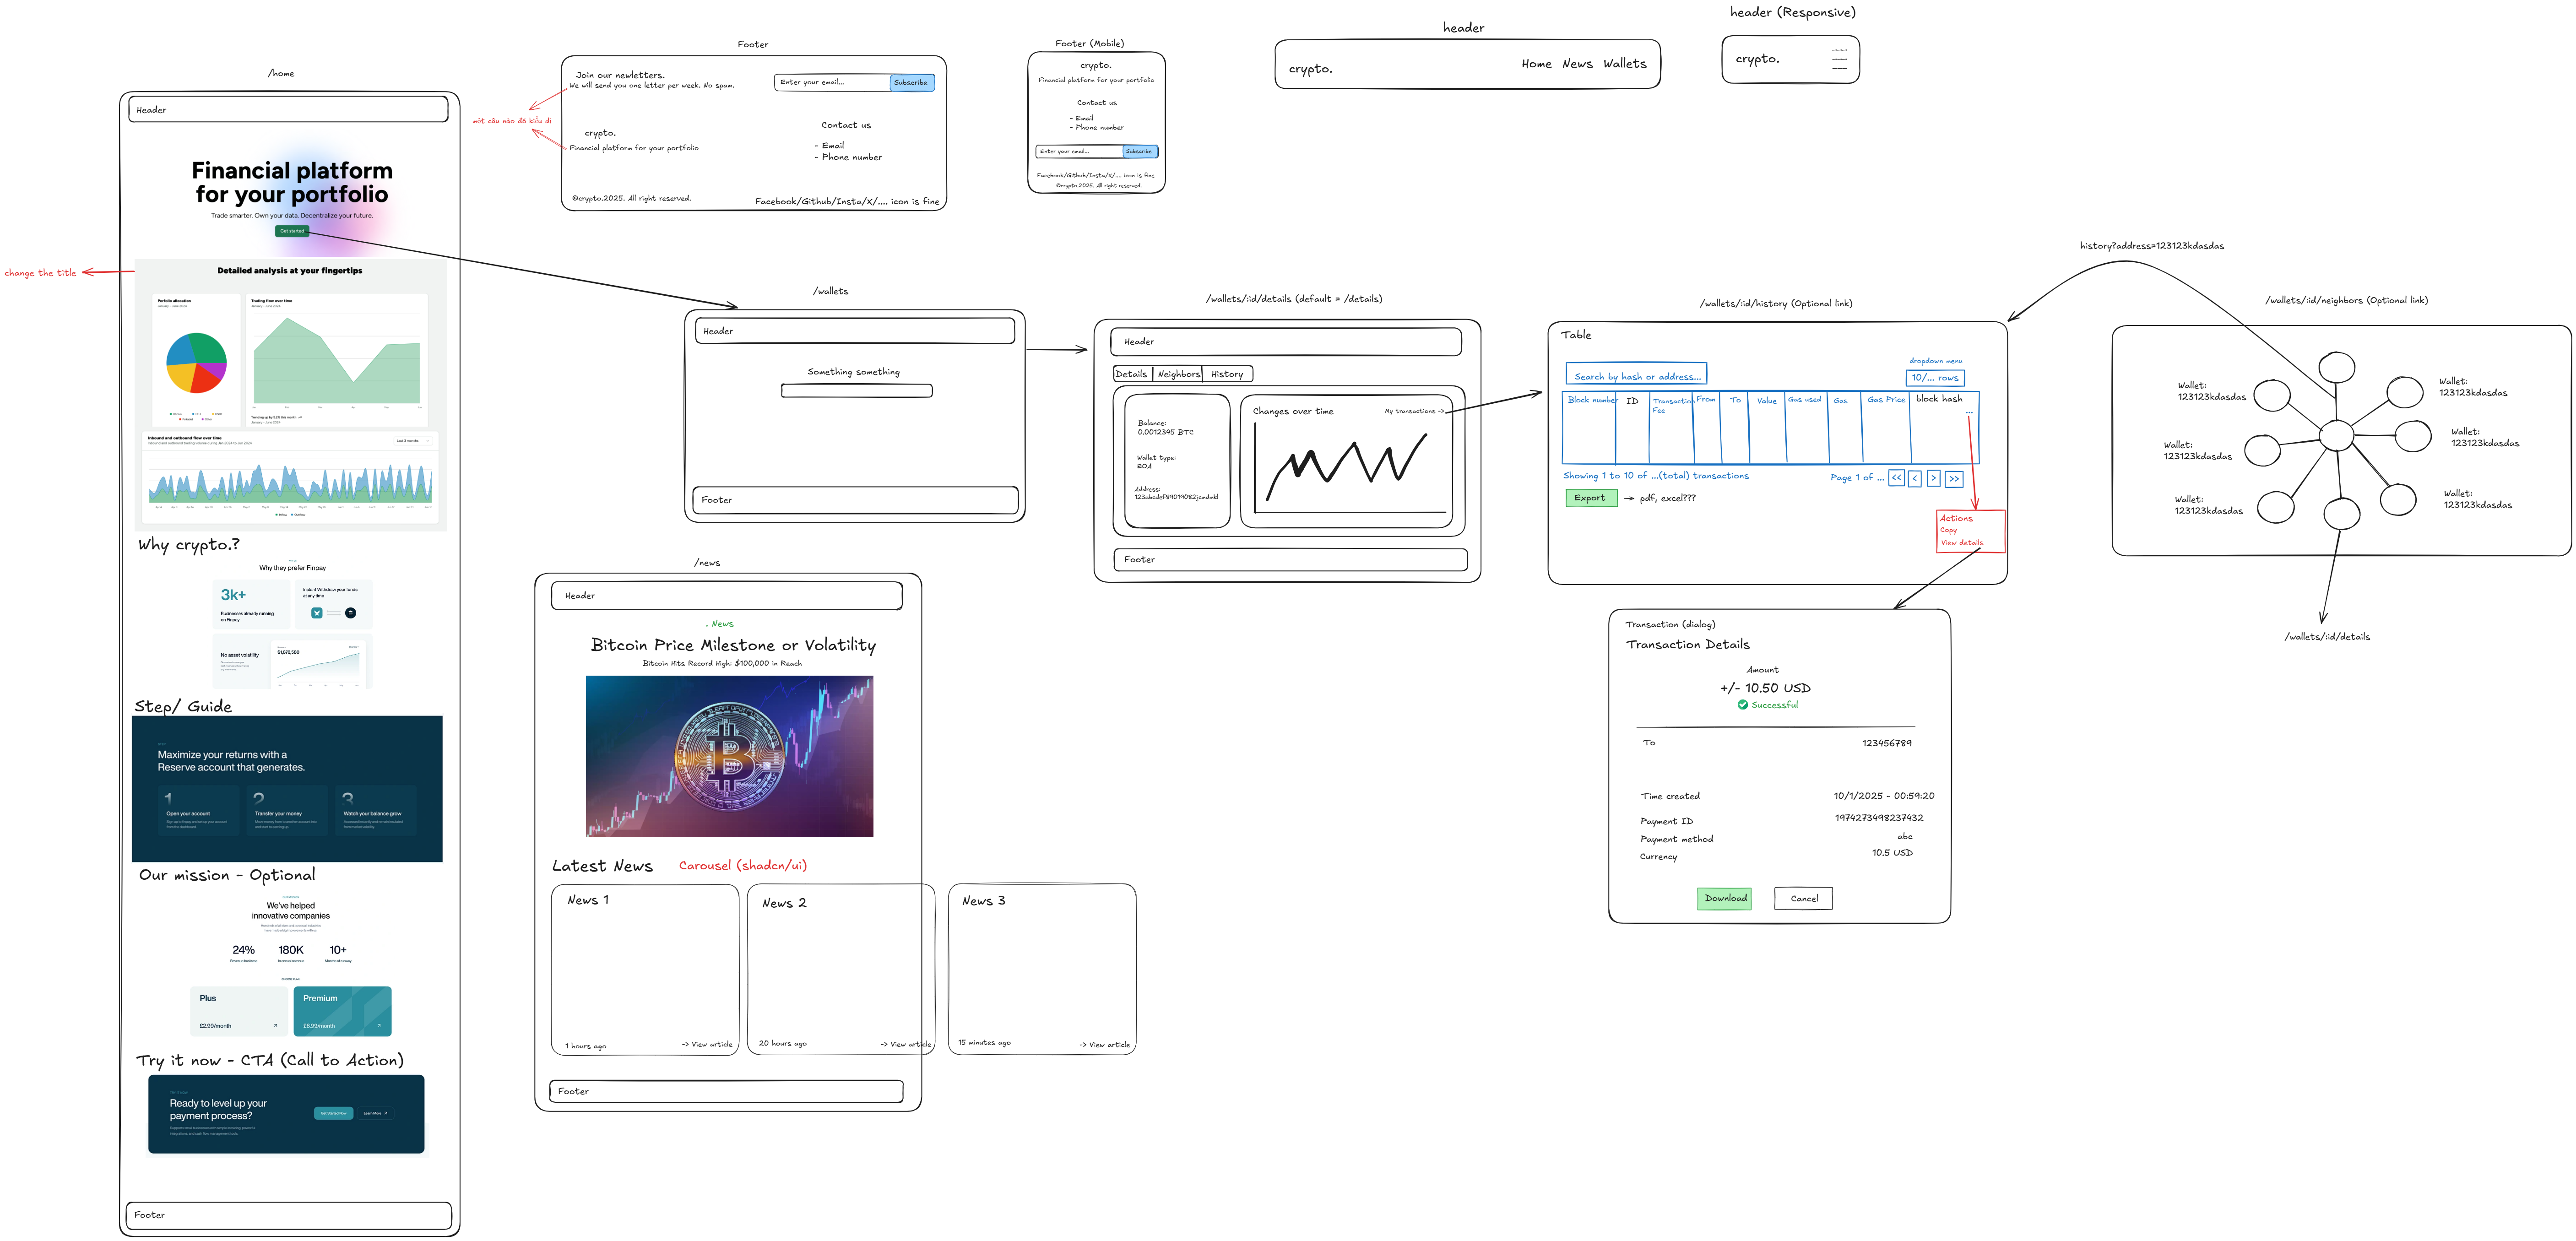
\includegraphics[width= 1\textwidth,  keepaspectratio]{root/image.png}
    \caption{Front-end prototype. \href{https://excalidraw.com/\#room=9d4fa2b42691ec469547,47-HCI7BFUW576wjGYaIXw}{Demo link}}
    \label{fig:prototype}
\end{figure}
\section{Design Principles}
The design principles for our platform (Figure \ref{fig:prototype}) establish a clean and efficient user experience through thoughtful minimalism and clear hierarchy. By removing unnecessary elements, the interface allows users to focus on essential features while maintaining intuitive navigation. The platform's responsive design ensures seamless adaptation across devices, from mobile phones to desktop computers, while maintaining visual consistency through unified elements like rounded corners and strategic whitespace. Professional typography and careful spacing work together to enhance readability and reinforce brand identity. These integrated design choices create a cohesive, trustworthy financial interface that balances functionality with refined aesthetics, delivering a professional experience that meets users' needs across all touchpoints.
\section{Prototype Explanation}
\subsection{Header and Footer}
 Header and footer will be implemented globally across our platform to  provide essential navigation, communication channels, and legal information in an organized and accessible manner, supporting the platform's overall user experience goals.
\begin{figure}[h]
    \centering
    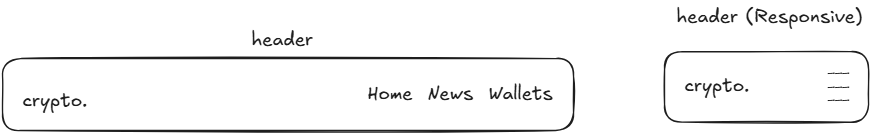
\includegraphics[width= 0.9\textwidth,  keepaspectratio]{root/header.png}
     \caption{Header}
    \label{fig:header}
\end{figure}
\paragraph{} The desktop header (Figure \ref{fig:header}) has a clean, minimalist design with "crypto." aligned to the left as the logo/brand name, and a horizontal navigation menu to the right containing three links: "Home," "News," and "Wallets." The responsive mobile version maintains the "crypto." branding on the left but replaces the navigation menu with a hamburger menu icon ($\equiv$) on the right, which is a common pattern for collapsing navigation options on smaller screens. Both headers appear to use a simple black and white color scheme with rounded rectangle borders containing the elements.
  \begin{figure}[h]
    \centering
    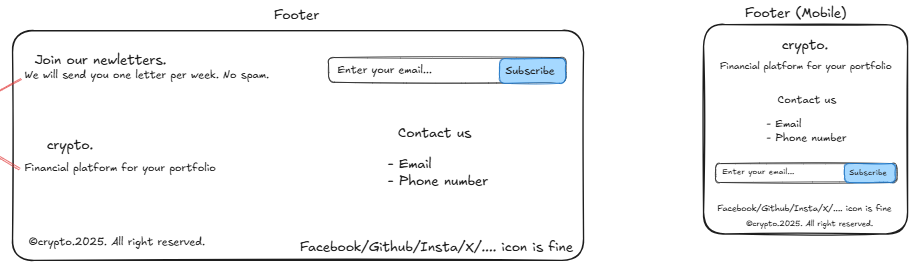
\includegraphics[width= 0.9\textwidth, keepaspectratio]{root/footer.png}
     \caption{Footer}
    \label{fig:footer}
\end{figure}
\paragraph{}The footer in Figure \ref{fig:footer} design demonstrates a thoughtful approach to responsive web design with desktop and mobile versions. The desktop layout spreads content horizontally, featuring a newsletter subscription section with a clear "no spam" promise, email input field, and a subscribe button. The company branding "crypto." appears with its descriptive tagline "Financial platform for your portfolio" alongside contact options for email and phone. Social media integration is indicated for platforms like Facebook, GitHub, Instagram, and X, though currently shown as text placeholders. The mobile version adapts this content into a vertical stack while maintaining all key elements, optimizing space usage for smaller screens. Both versions include the copyright notice "crypto.2025. All right reserved." and share a consistent minimalist black and white color scheme, ensuring a cohesive user experience across devices.
\subsection{Homepage}
\begin{figure}[h]
    \centering
     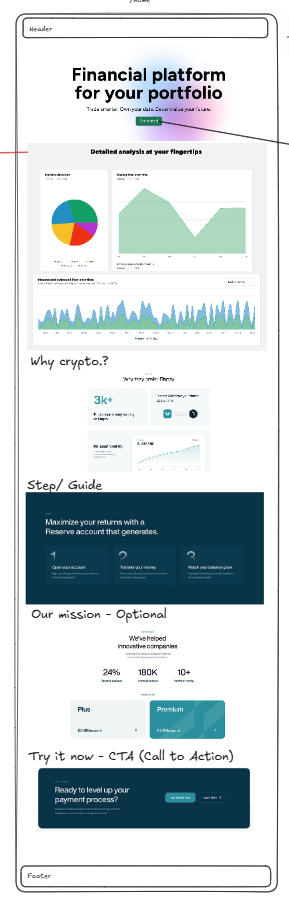
\includegraphics[width= \textwidth, height=0.595\textheight, keepaspectratio]{root/homepage.png}
    \caption{Homepage}
    \label{fig:homepage}
\end{figure}
\paragraph{}Our homepage (Figure \ref{fig:homepage}) embodies a user-centric design philosophy, emphasizing minimalism and intuitive navigation. The layout is strategically segmented into distinct functional sections that serve dual purposes: showcasing our system's core capabilities while providing a clear onboarding path for new users. Each section is thoughtfully crafted to maintain visual hierarchy and guide visitors through a seamless exploration of our platform.
  \begin{figure}[h]
    \centering
    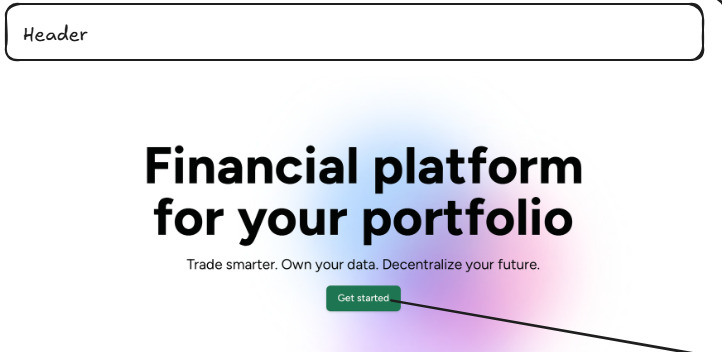
\includegraphics[width= 0.8\textwidth, keepaspectratio]{root/hero.png}
     \caption{Hero section}
    \label{fig:hero}
\end{figure}
\paragraph{}The homepage prototype begins with a clean and modern header section ( see Figure \ref{fig:hero}). Below it, the hero section showcases a bold headline "Financial platform for your portfolio" against a crisp white background. This background is artfully decorated with three floating spherical elements in different colors, creating a subtle but dynamic visual interest. The spheres appear to be gently moving in the space, adding a touch of playfulness to the professional design. A prominent green call-to-action button stands out beneath the headline, inviting users to begin their journey with the platform. The entire hero section effectively combines simplicity with visual appeal, immediately communicating the platform's purpose while maintaining an engaging and modern aesthetic.
 \begin{figure}[h]
    \centering
    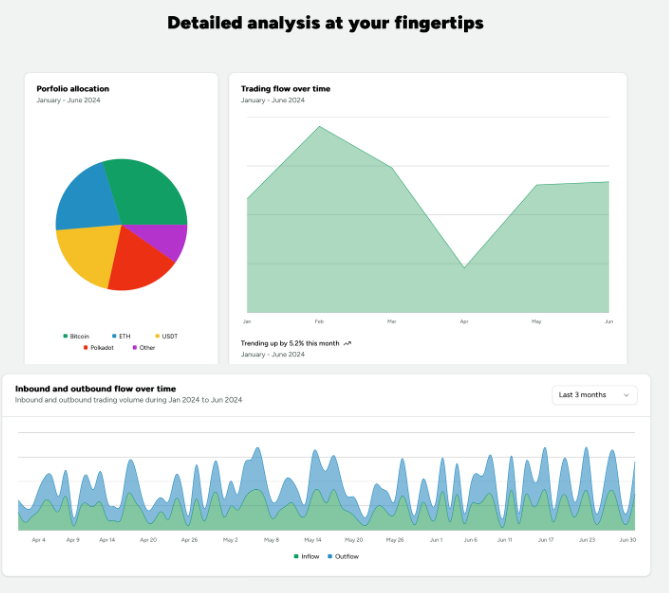
\includegraphics[width= 0.9\textwidth, 
    height=0.6\textheight, keepaspectratio]{root/analysis.png}
     \caption{Visualizations}
    \label{fig:analysis}
\end{figure}

\paragraph{}Next part of the homepage is the dashboard section (Figure \ref{fig:analysis}). This section showcases three distinct visualization types - a pie chart representing portfolio allocation, an area chart displaying trading flow trends, and a detailed inbound/outbound flow graph - providing potential users with a comprehensive preview of the platform's analytical capabilities. These interactive visualizations serve as a powerful demonstration of the system's ability to transform complex blockchain transaction data into clear, actionable insights, allowing visitors to immediately grasp the platform's value proposition. The visualizations employ a minimalist design approach with a professional color scheme of soft greens and blues, complemented by strategic accent colors. The layout features a clean grid system with balanced spacing and subtle shadows, while clear sans-serif typography maintains information hierarchy. Interactive elements like time period selectors and smooth transitions enhance user engagement, all while maintaining a sophisticated yet approachable aesthetic that makes complex financial data easily digestible.
 \begin{figure}[h]
    \centering
    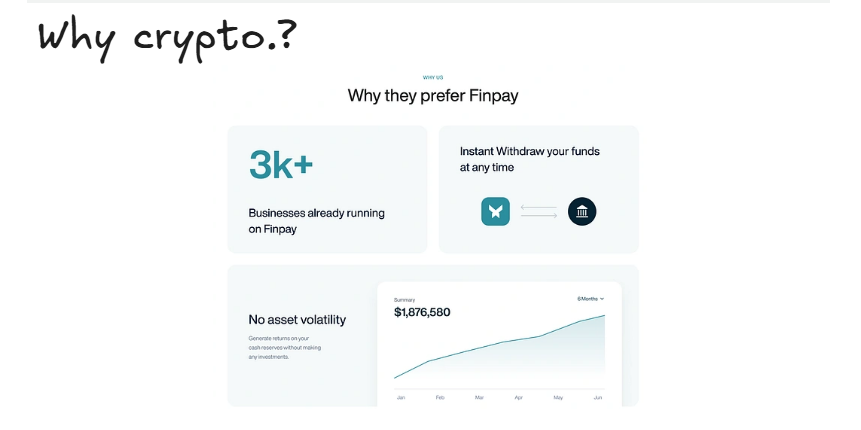
\includegraphics[width= 0.9\textwidth, keepaspectratio]{root/why.png}
     \caption{Why Choose Us page layout}
    \label{fig:Why choose us}
\end{figure}
\paragraph{}In this "Why Choose Us" section (see Figure \ref{fig:Why choose us}), we address typical concerns about cryptocurrency trading while highlighting our key strengths through a streamlined, intuitive interface. Our clean, minimalist design approach makes complex trading concepts more approachable, while reinforcing user confidence through visual clarity. Features are displayed in harmoniously styled cards, creating a cohesive visual narrative that emphasizes both professionalism and ease of use. This carefully structured presentation helps demystify cryptocurrency trading for newcomers while offering the depth that experienced traders expect, with each benefit clearly articulated to demonstrate our platform's value.
\begin{figure}[h]
    \centering
    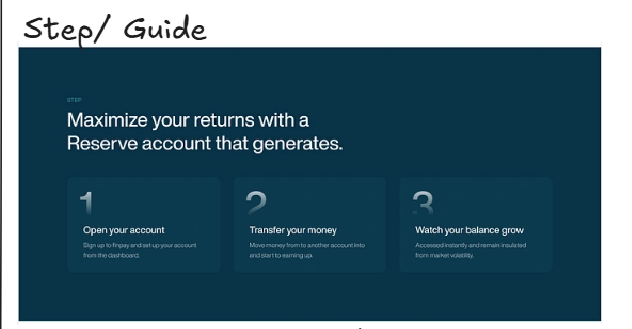
\includegraphics[width= 0.9\textwidth]{root/step.png}
     \caption{Guide for users to start}
    \label{fig:step}
\end{figure}
\paragraph{}The homepage continues with tutorial sections (Figure \ref{fig:step}), which showcase a meticulously designed onboarding section for cryptocurrency trading, featuring a streamlined three-step process presented in a sophisticated dark-themed interface. The intuitive design hierarchy, led by a compelling and appropriate headline, guides users through essential stages: wallet creation, account funding, and trading initiation. Each step is thoughtfully presented with consistent visual elements, including numbered cards, descriptive text, and thematic icons in an engaging green accent color. The clean layout and clear information architecture effectively communicate both simplicity and professionalism, while the "Learn more" links provide depth as well as clear tutorial without overwhelming new users. This design aims to balance the complexity of cryptocurrency trading with an approachable user experience, making it particularly effective for both newcomers and experienced traders looking for a straightforward platform.

\paragraph{} The "Our Mission" section (refer to \ref{fig:option}) presents a thoughtfully designed pricing and impact showcase that effectively combines social proof with subscription options. The layout employs a clean, hierarchical structure beginning with impressive statistics, which immediately establishes credibility and scale of impact. Below these metrics, the section transitions smoothly into a dual-tier pricing structure featuring "Plus" and "Premium" plans, priced at \pounds 2.99 and \pounds 5.99 per month respectively. The design utilizes a subtle yet effective color contrast, with the Premium tier highlighted in a professional teal color against the Plus tier's neutral background, subtly guiding users toward the higher-value option. The pricing cards maintain a clean, minimalist approach with clear monthly pricing and directional arrows, making the selection process straightforward and uncluttered. This section successfully balances social proof with commercial offerings, while the "Optional" notation suggests flexibility in implementation, allowing for strategic placement within the broader platform design.
\begin{figure}[h]
    \centering
    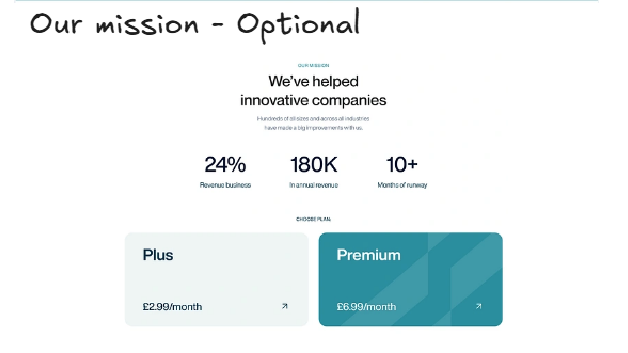
\includegraphics[width= 0.9\textwidth]{root/option.png}
     \caption{Pricing plan and impact showcase}
    \label{fig:option}
\end{figure}
\paragraph{} The Call-to-Action (CTA) section, see Figure \ref{fig:cta}, displays a sophisticated and compelling design approach within a deep navy-colored banner that draws immediate attention. The section will lead with an engaging question, for example "Ready to level up your payment process?", which creates a direct connection with potential users while highlighting the platform's core value proposition. The layout will employ a clean, horizontal structure with a supporting subheading that emphasizes business benefits and management tools. Two distinct action buttons - "Get Started Now" and "Learn More" - provide clear pathways for users at different stages of the decision-making process, with the primary CTA featuring a contrasting color to drive conversions. The dark background paired with light text creates strong visual contrast, ensuring readability while maintaining a professional, fintech-appropriate aesthetic. This CTA section effectively balances urgency with professionalism, using strategic spacing and typography to create a clean, uncluttered call to action that encourages user engagement without appearing overly aggressive.
\begin{figure}[h]
    \centering
    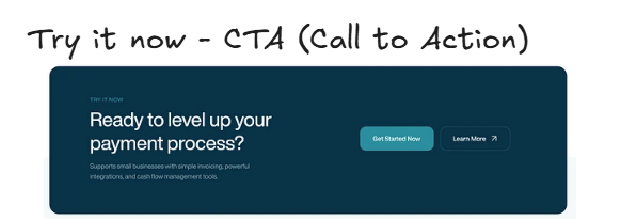
\includegraphics[width= 0.9\textwidth]{root/cta.png}
     \caption{Call to action}
    \label{fig:cta}
\end{figure}
\paragraph{}This compelling Call-to-Action section serves as the homepage's final touchpoint, strategically positioned immediately above the footer. Acting as a powerful closing statement, it provides a clear pathway for user conversion while maintaining the sleek, professional aesthetic established throughout the page.

\subsection{News page}
\begin{figure}[h]
    \centering
    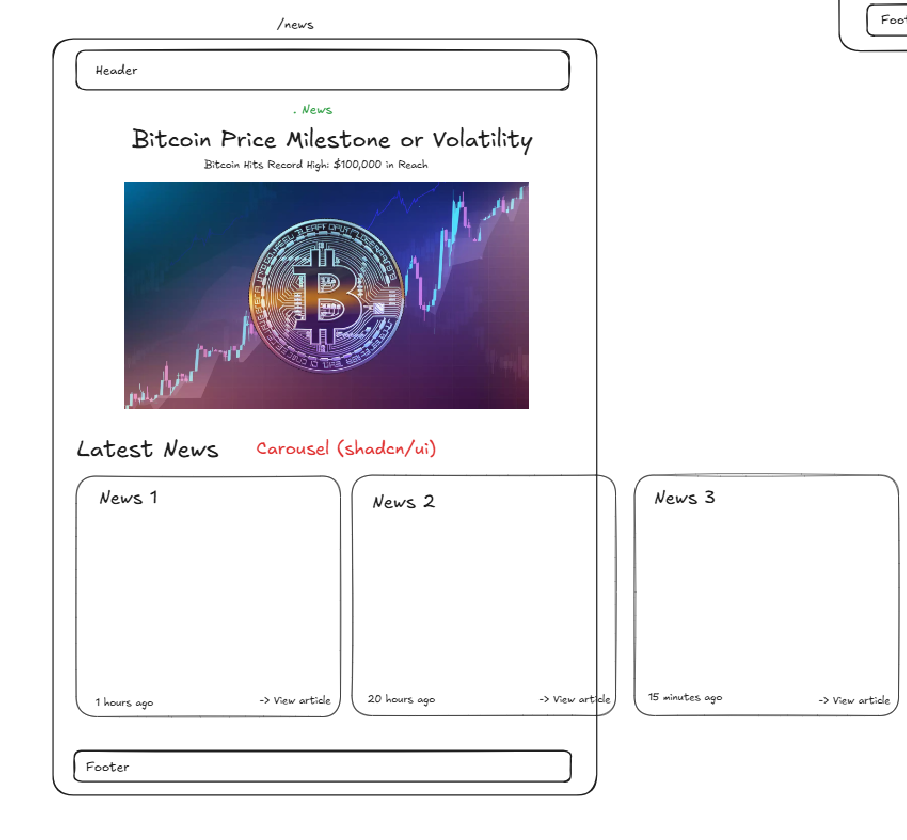
\includegraphics[width= 0.8\textwidth, height=0.6\textheight]{root/news.png}
     \caption{News page}
    \label{fig:news}
\end{figure}
\paragraph{}This news page design showcases a thoughtfully structured layout that effectively delivers cryptocurrency news content through a clear visual hierarchy. The page opens with a prominent header containing navigation links, leading into a featured story section that commands attention .Below, a "Latest News" carousel implemented using shadcn/ui components displays three news cards, each featuring timestamps and "View article" links, creating a dynamic flow of information. The design maintains professional credibility while ensuring easy navigation, with clear timestamps, providing content recency, and consistent spacing throughout the layout enhancing readability.
\subsection{Wallets page}
\paragraph{}When users navigate to the Wallets page (Figure \ref{fig:search}), they will land on a screen featuring a search bar. By entering a wallet address into this search bar, users can retrieve and view the detailed information associated with that specific wallet.
\begin{figure}[h]
    \centering
    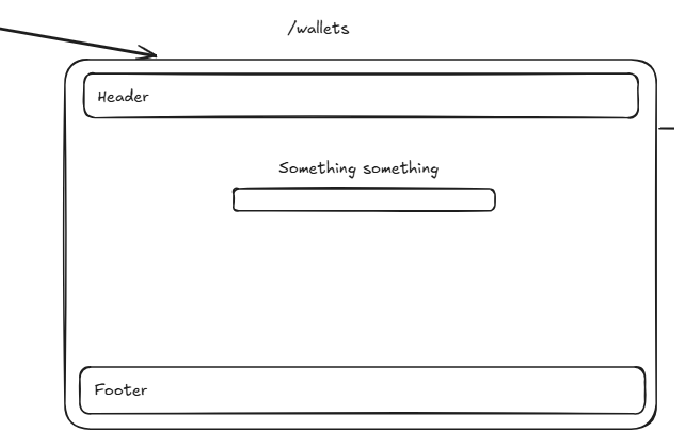
\includegraphics[width= 0.6\textwidth, keepaspectratio]{root/search.png}
     \caption{Search page}
    \label{fig:search}
\end{figure}
\paragraph{}After entering a correct wallet address, users will be navigated to wallet details page (Figure \ref{fig:Wallet_Detail}), accessed via the route /wallets/:id/details. The design of this page employs a traditional web application structure with header and footer elements framing the main content area. The interface features a prominent three-tab navigation system (Details, Neighbors, History), with Details serving as the default view. The main content is thoughtfully divided into two primary panels: the left panel displays essential wallet information including the BTC balance (0.0012345 BTC), wallet type (EOA), and a truncated wallet address, while the right panel showcases a dynamic line graph titled "Changes over time" that visualizes transaction or value history with notable fluctuations.
\begin{figure}[h]
    \centering
    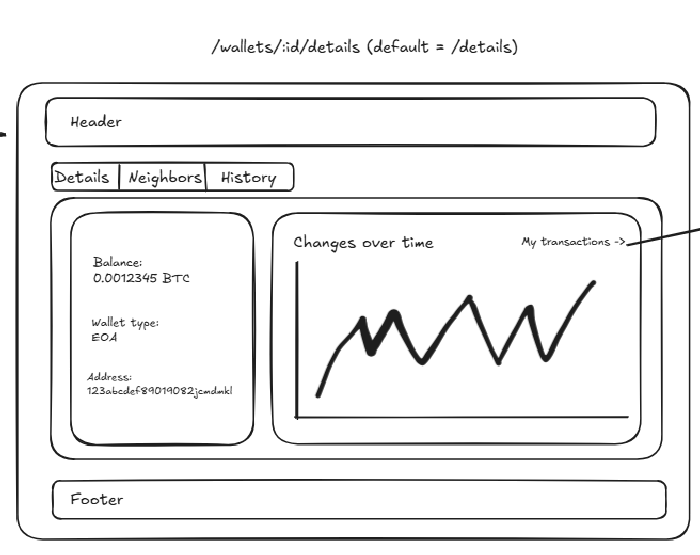
\includegraphics[width= 0.6\textwidth, keepaspectratio]{root/wallet_wallets.png}
     \caption{Wallet Details}
    \label{fig:Wallet_Detail}
\end{figure}
\paragraph{} The Wallet Pages include ``My Transactions'' and ``History'' options in the navigation bar (Figure \ref{fig:Wallet_Detail}). Clicking either of these options takes the user to a comprehensive view of the transaction history, refer to Figure \ref{fig:history}, for the selected wallet.

To enhance usability, the transaction history table incorporates several practical features:

\begin{itemize}
  \item \textbf{Search bar:} Allows filtering transactions by hash or address
  \item \textbf{Pagination:} Enables navigating through transaction records page by page
  \item \textbf{Export options:} Supports exporting transaction data in PDF or Excel file formats
\end{itemize}

Selecting an individual transaction from the table opens a detailed transaction dialog window. This dialog provides in-depth information about the selected transaction, such as:

\begin{itemize}
  \item Precise date and time of the transaction
  \item Associated payment IDs
  \item Exact transaction amounts
  \item Clear success/failure status indicators
\end{itemize}

This thoughtfully designed combination of a comprehensive transaction history table and detailed drill-down dialogs empowers users to easily navigate, analyze, and manage their wallet's transaction records.
\begin{figure}[h!]
    \centering
    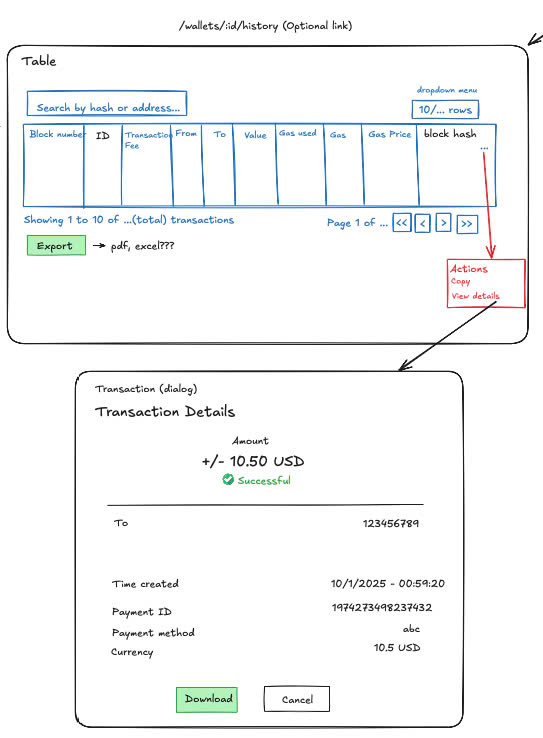
\includegraphics[width= 0.5\textwidth, height=0.73\textheight, keepaspectratio]{figures/test.jpg}
     \caption{Wallet Transaction History}
    \label{fig:history}
\end{figure}

\paragraph{} The /wallets/id/neighbors page (Figure \ref{fig:graph}) displays an interactive network visualization that shows how different wallets are connected through transactions. In this graph, each point (or node) represents a unique wallet address.  This interactive visualization allows users to explore and analyze transactions by clicking on nodes or edges to view specific details such as transaction amounts, timestamps, and associated metadata (transaction details in a table on the /wallets/id/history), see Figure \ref{fig:history}. Each wallet node is labeled with an unique wallet address.

\paragraph{}But why we need to add this graph visualization to our platform? Incorporating this visualization into our blockchain visualization platform offers several benefits. It enables users to easily explore and trace the flow of funds, potentially detecting suspicious activities or anomalies indicative of fraud or money laundering. The graph provides insights into wallet connectivity and relationships, identifying central wallets acting as transaction hubs and discovering closely connected wallet communities. Also, the user-friendly visual representation enhances transparency and accessibility, making it easier for users to understand and trace fund movements without delving into complex raw transaction data.

\begin{figure}[H]
    \centering
    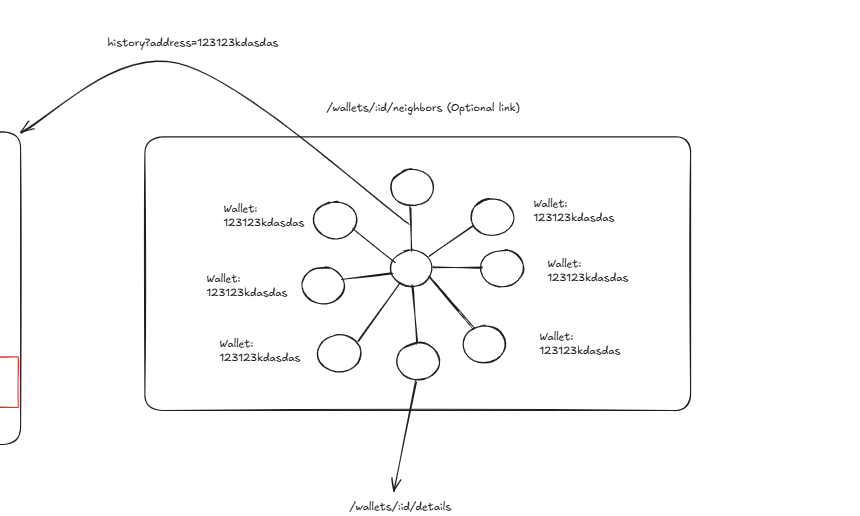
\includegraphics[width= 0.7\textwidth]{root/graph.png}
     \caption{Transactions Depicted in Graph Format}
    \label{fig:graph}
\end{figure}





 
 


\chapter{Prototype to Deployment} \label{ch5}
\paragraph{} The process of implementing the front-end from prototype to deployment is not only an exciting journey, but it is also a process filled with valuable learning experiences for our development team. During this phase, we have acquired new knowledge and skills while fine-tuning and refining the project to ensure optimal performance and suitability. As a result, the official website has undergone several improvements and enhancements compared to the prototype version. In this section of the report, we will highlight the key areas where we have made significant improvements to the project.
\paragraph{}First and foremost, after the hero section, we showcase logos of major tech companies (Figure \ref{fig:logos}) that use our platform, helping build trust and credibility with potential users.
  \begin{figure}[h]
    \centering
    
\includegraphics[width= 1\textwidth]{figures/deploy_change.png}
     \caption{Company logos}
    \label{fig:logos}
\end{figure}
\paragraph{}We redesigned the "Why crypto?" section (see Figure \ref{fig:Why choose us}) to improve readability by adding more spacing between cards, making it more visually appealing than our previous layout. We added the headline "Trade crypto with confidence" to inspire trust and enthusiasm among potential users. We also made a deliberate choice to use "Why Choose Us?" (Figure \ref{fig:Why_choose_us_2.0}) instead of "Why crypto?"(see Figure \ref{fig:Why choose us}) as we believe this phrasing creates a more personal connection with users and emphasizes our community-focused approach, which helps build trust in our platform. We enhanced the section's key messages by using bolder, darker fonts that contrast well against the light background. This makes our core ideas immediately stand out and easier for users to grasp at first glance.
  \begin{figure}[h]
    \centering
    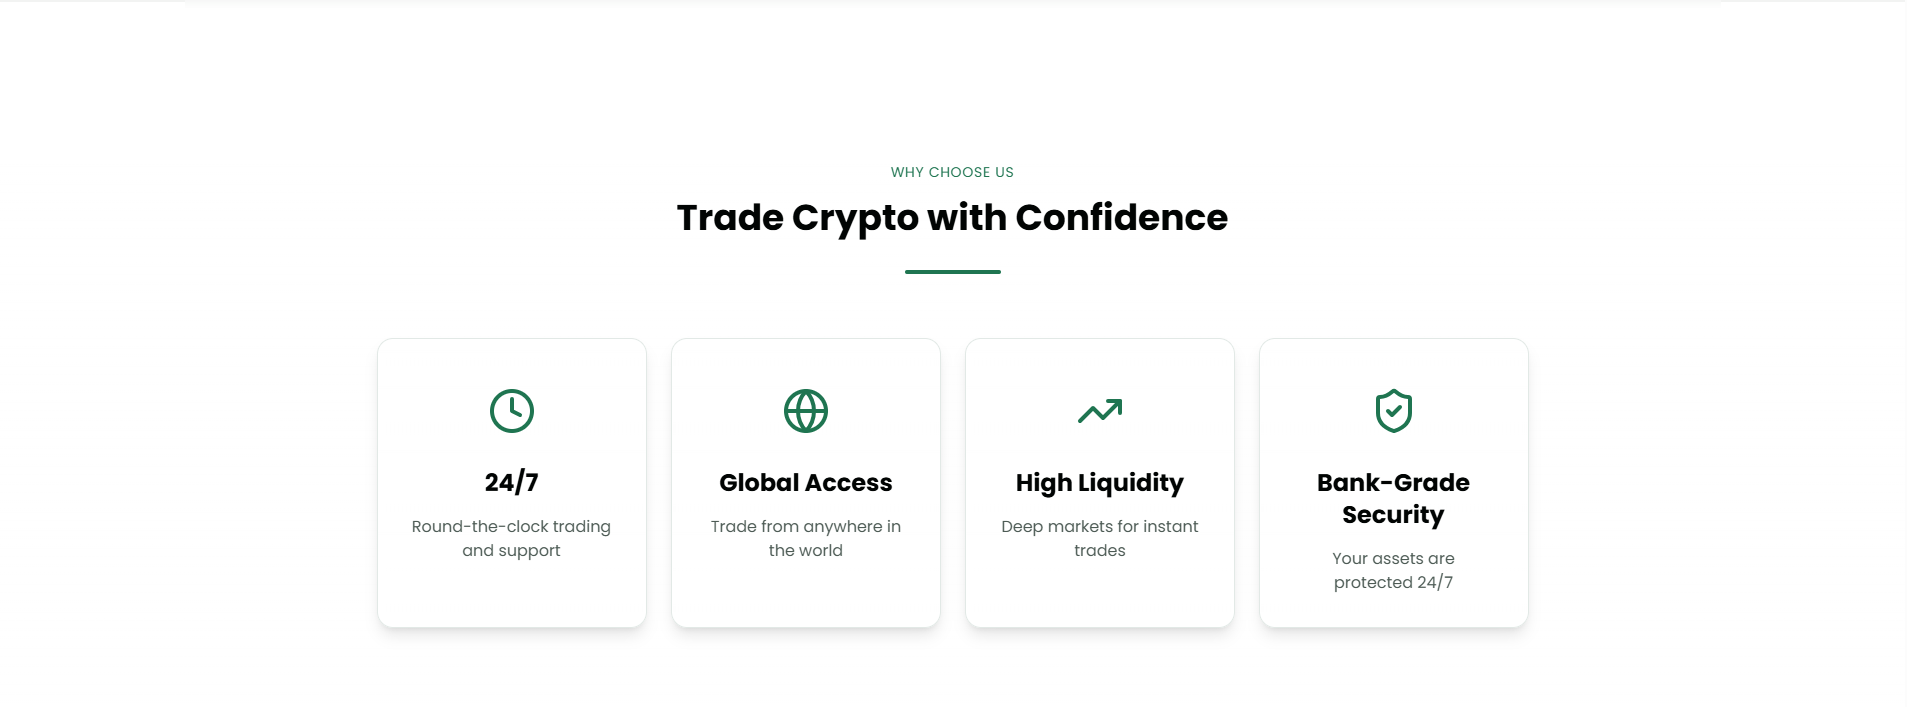
\includegraphics[width= 1\textwidth]{figures/deploy_change_2.png}
     \caption{Official Why choose us?}
    \label{fig:Why_choose_us_2.0}
\end{figure}
\paragraph{} In revamping the tutorial section, we moved away from our prototype's softer design (see Figure \ref{fig:step}) to better reflect cryptocurrency's cutting-edge nature, Figure \ref{fig:step_2.0}. We implemented a more modern aesthetic by using bold, dark backgrounds with white text, creating a sleek, tech-forward appearance. The instructions were also streamlined with shorter, more concise text to create a more user-friendly guide for newcomers.
  \begin{figure}[h]
    \centering
    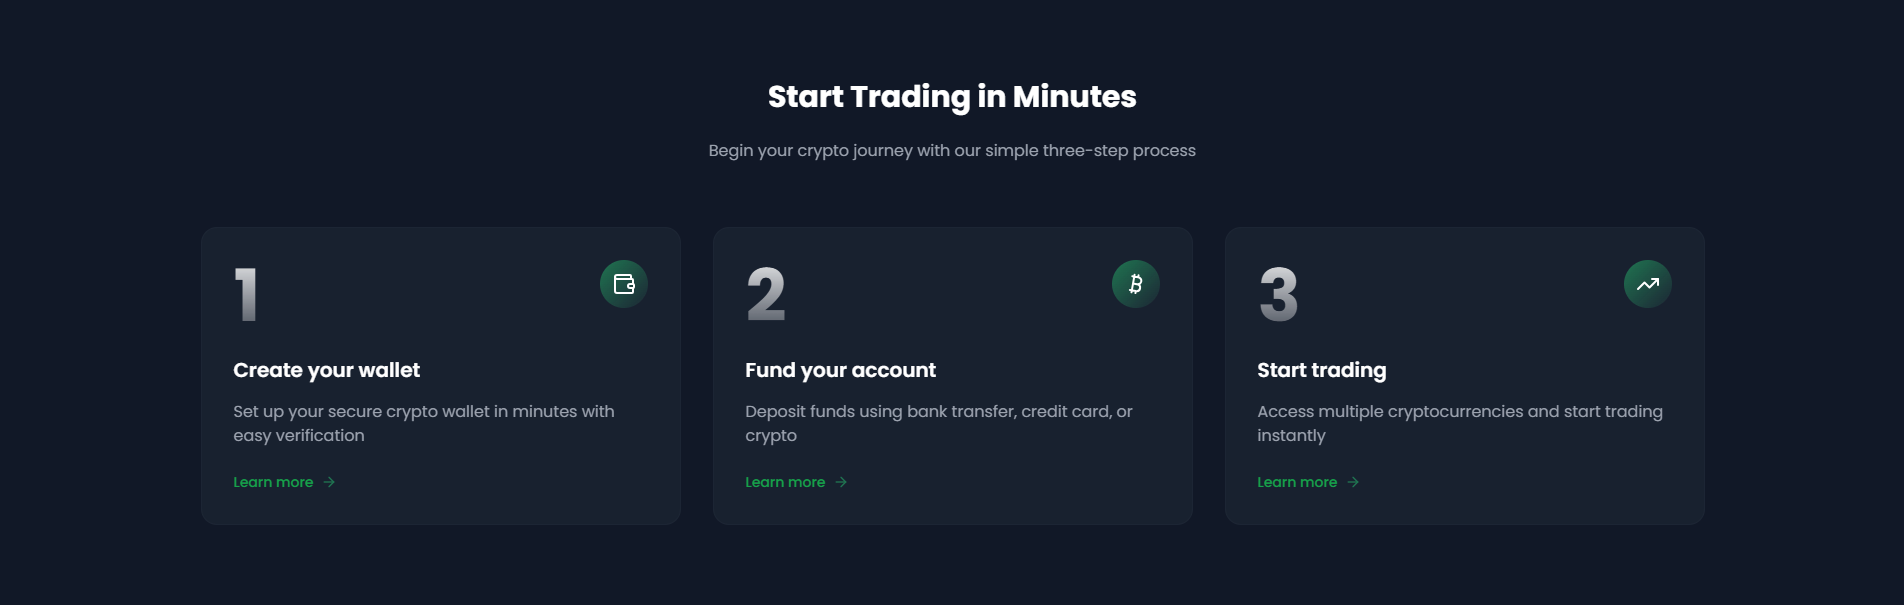
\includegraphics[width= 0.9\textwidth, keepaspectratio]{figures/Screenshot 2025-02-16 154618.png}
     \caption{Official Guide for users to start}
    \label{fig:step_2.0}
\end{figure}
\paragraph{}We simplified the mission section (see Figure \ref{fig:option}) by removing excess text and creating more white space. Instead, we now highlight key statistics about our platform's achievements, which demonstrate both our strong presence in the crypto trading community and our track record of consistent performance. This streamlined approach makes our success metrics more prominent and impactful. Those changed resulted in our new mission section, Figure \ref{fig:option_2.0}
  \begin{figure}[h]
    \centering
    
\includegraphics[width= 1\textwidth]{root/op1.png}
     \caption{Official Mission section}
    \label{fig:option_2.0}
\end{figure}
\paragraph{}We introduced a new free tier to our pricing structure to make our platform accessible to a wider range of users, from beginners to professional traders and organizations. Each pricing plan is carefully tailored to match different user needs and usage levels, ensuring that every customer segment finds an appropriate and cost-effective option for their trading activities.
  \begin{figure}[h]
    \centering
    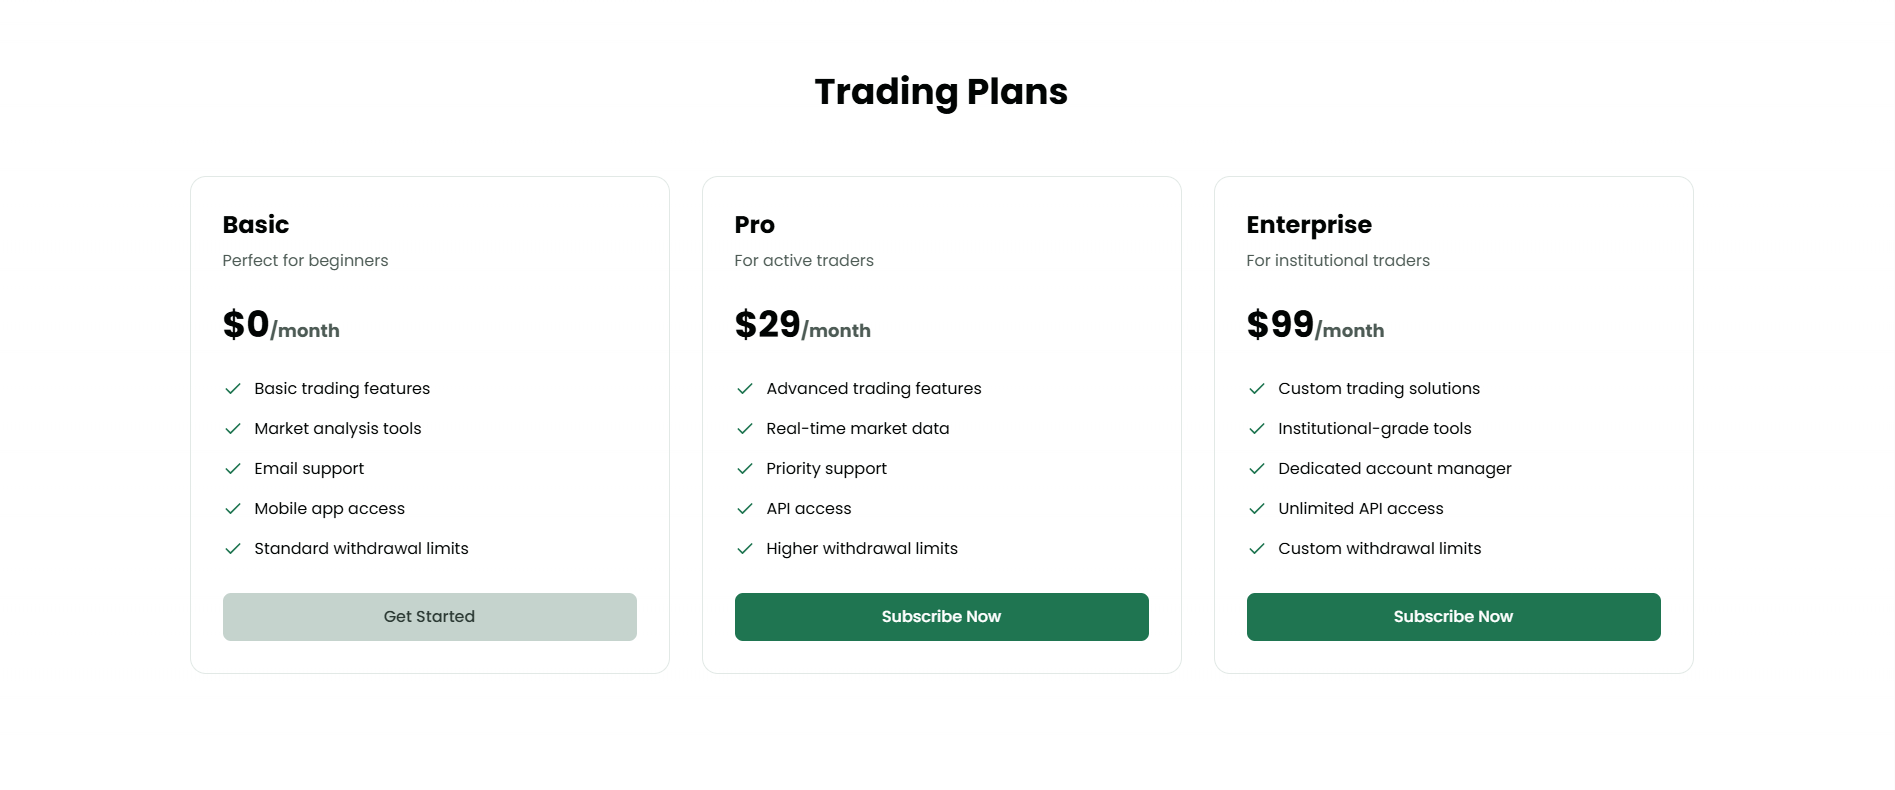
\includegraphics[width= 1\textwidth]{root/op2.png}
     \caption{Official Pricing Plan}
    \label{fig:option_2_2.0}
\end{figure}
\paragraph{} Lastly is our platform's "Try it out" section's transformation.The section underwent a complete strategic overhaul. Instead of focusing narrowly on payment processing for small businesses, we broadened our message to "Start Your Journey Today," positioning ourselves as a comprehensive global trading platform. To build credibility, we now showcase our key achievements: over \$2 billion in trading volume, operations in more than 180 countries, and a million-plus user base.
The design also evolved significantly, replacing the simple teal color scheme with a more sophisticated dark theme accented with green. We now prominently highlight crucial features like bank-grade encryption and high-speed transactions, addressing key user concerns about security and performance. The call-to-action button was also refined from a generic "Learn More" to a more action-oriented "View Pricing Plans," creating a clearer path for potential users.
 \begin{figure}[h]
    \centering
    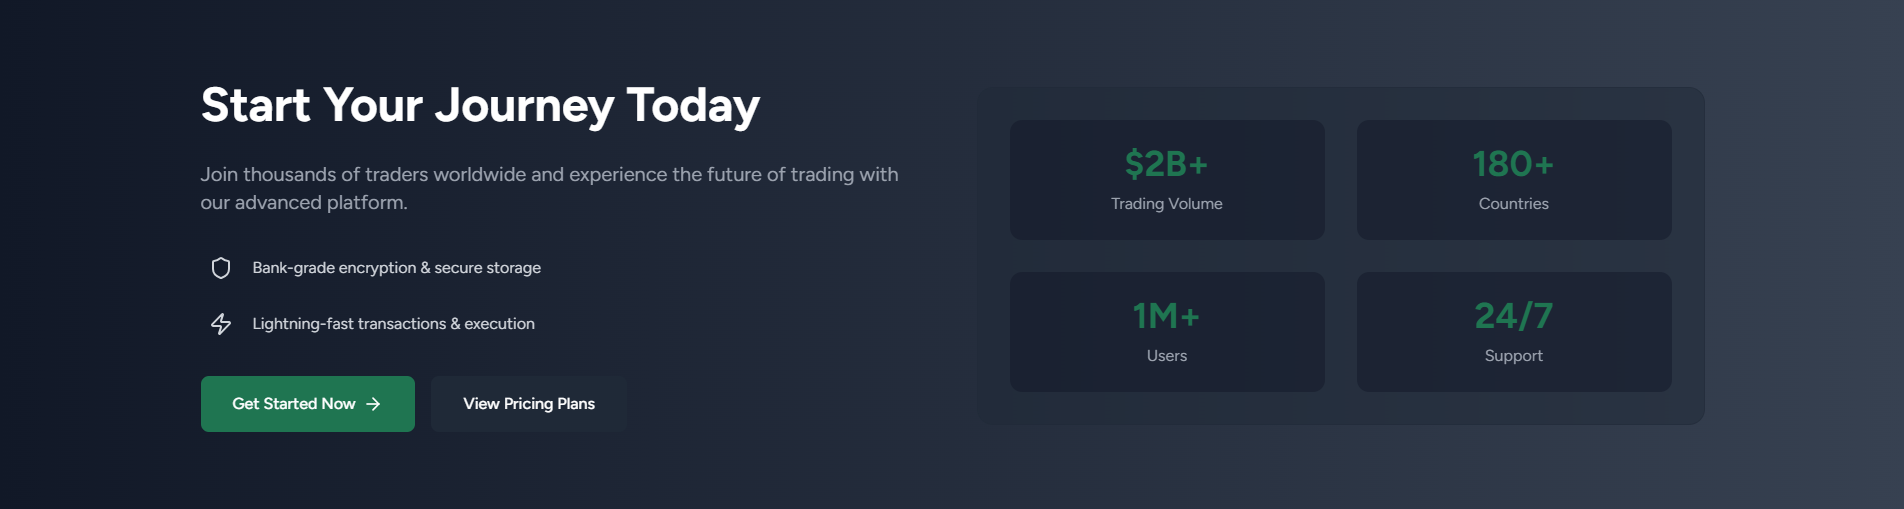
\includegraphics[width= 1\textwidth]{root/cta_2.png}
     \caption{Official Call-To-Action}
    \label{fig:cta_2.0}
\end{figure}
\paragraph{} The main component of my webpage is Wallets where users can keep track with their wallets' transaction information and activity. The search page of ./Wallets design stay unchanged compared to prototype, Figure \ref{fig:search}. Below the official search page:
 \begin{figure}[h]
    \centering
    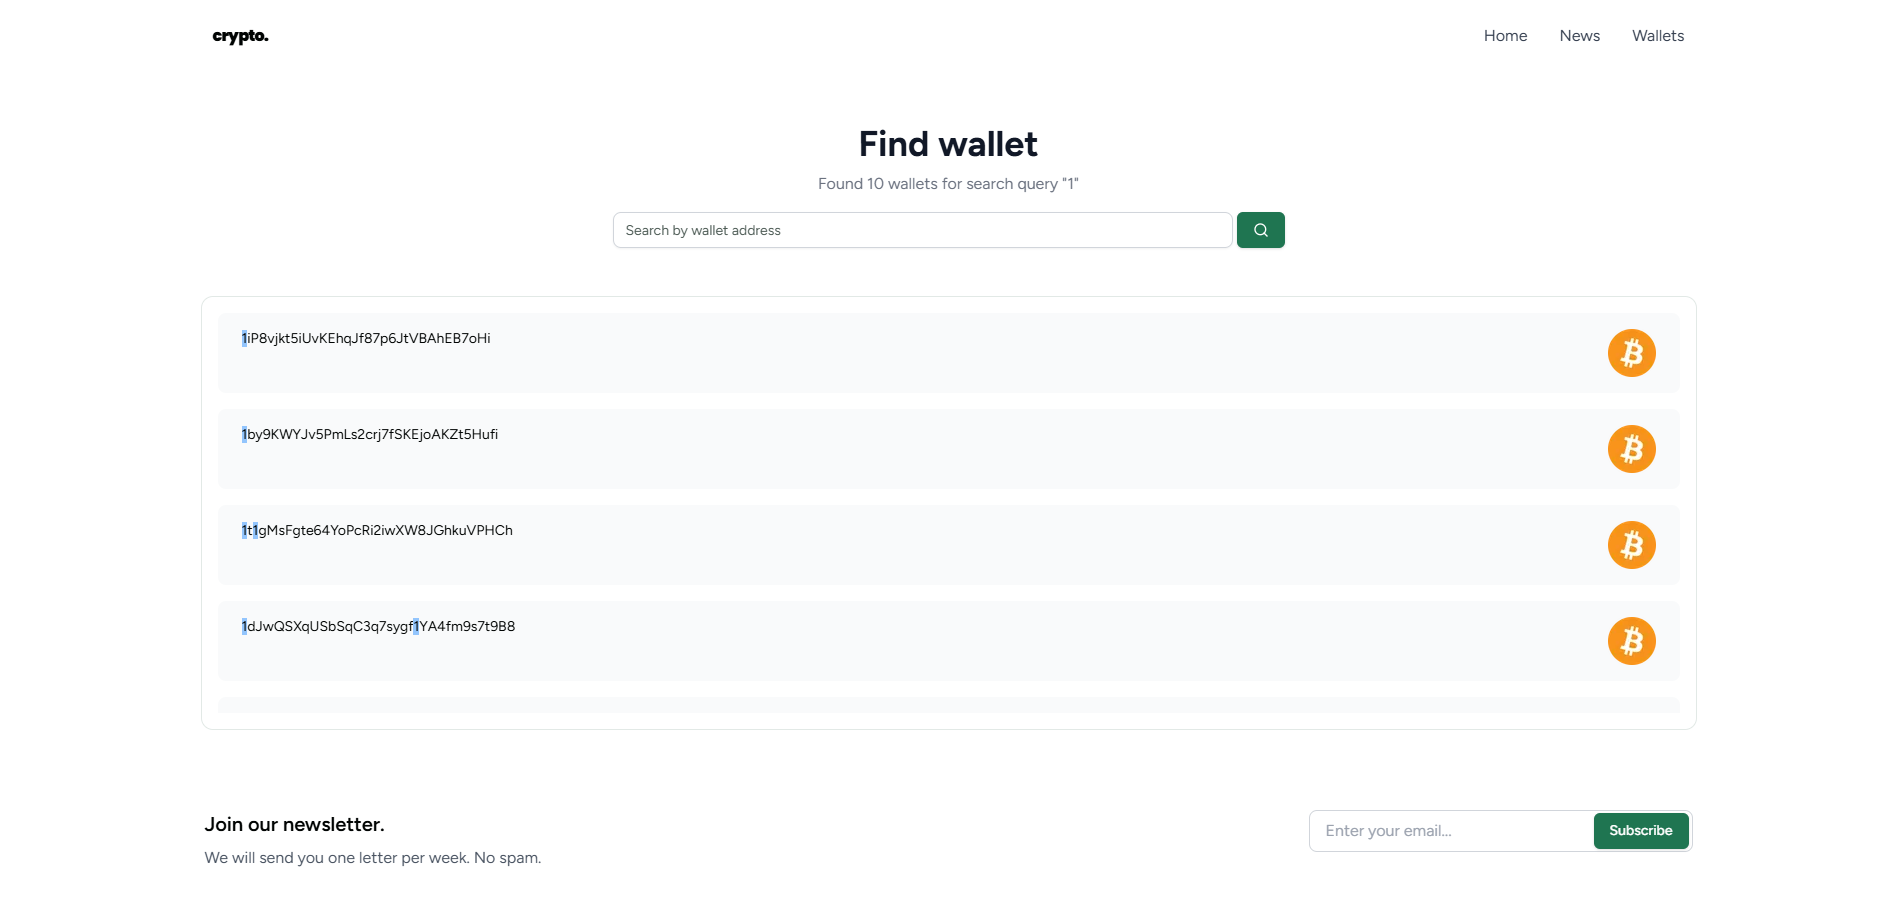
\includegraphics[width= 1\textwidth]{root/wallet_search.png}
     \caption{Official ./wallets}
    \label{fig:wallet_search}
\end{figure}
\paragraph{} The Wallet Details page (/wallets/:id/details) has been streamlined by removing the right panel that was intended to display a "Changes Over Time" line graph (refer to \ref{fig:Wallet_Detail}). This feature was removed because our team encountered significant implementation challenges and decided to postpone its development rather than delay the platform's launch. Similarly, the Transaction History page (/wallets/:id/history) has been simplified, with some transaction details being omitted from the original prototype to improve performance in this development phase.

\paragraph{} Throughout the development process, we have made strategic modifications to enhance performance and maintain consistency, resulting in some differences from our initial prototype. While certain features have been streamlined in this release, our team remains committed to advancing the platform's capabilities. We envision future iterations of our blockchain transaction visualization system incorporating more sophisticated features and technological breakthroughs, further enriching the user experience and functionality.





\section{Technical Decisions} \label{ch6}
\subsection{Front-end Technology Choices}

\subsubsection{Next.js}
Our front-end stack is built with Next.js, offering:
\begin{itemize}
    \item \textbf{Server-side Rendering:} Enhances SEO and initial page load performance
    \item \textbf{Static Generation:} Enables pre-rendering of static content
    \item \textbf{Advanced Routing:} Simplifies navigation with built-in file-based routing
    \item \textbf{App Directory:} Leverages new features like layouts and metadata management
\end{itemize}

\subsubsection{React \& TypeScript}
The combination of React and TypeScript provides:
\begin{itemize}
    \item \textbf{Component Architecture:} Modular, reusable UI components
    \item \textbf{Type Safety:} Robust type checking reducing runtime errors
    \item \textbf{Developer Tools:} Enhanced IDE support and code navigation
    \item \textbf{Code Maintainability:} Clear interfaces and improved documentation
\end{itemize}

\subsubsection{Tailwind CSS}
For styling, we chose Tailwind CSS because it offers:
\begin{itemize}
    \item \textbf{Utility-First Approach:} Rapid UI development with pre-built classes
    \item \textbf{Customization:} Flexible design tokens and CSS variables
    \item \textbf{Performance:} Built-in purging of unused styles
    \item \textbf{Consistency:} Standardized design system across components
\end{itemize}

\subsubsection{API Typesafety}

We use OpenAPI TypeScript code generation for API type safety:
\begin{itemize}
    \item \textbf{OpenAPI TypeScript Generation:} Using openapi-typescript to generate types from our backend Swagger documentation
    \item \textbf{Automated Type Updates:} Script "typegen" runs with tsx to regenerate types when API changes
    \item \textbf{Type Integration:} Generated types are imported and used throughout the frontend codebase
    \item \textbf{End-to-end Type Safety:} Ensures API requests and responses match backend specifications
\end{itemize}

The process involves:
\begin{itemize}
    \item \textbf{Step 1:} Running "typegen" script that fetches OpenAPI schema from backend
    \item \textbf{Step 2:} Converting schema to TypeScript interfaces automatically
    \item \textbf{Step 3:} Using generated types in API calls and components
\end{itemize}

\subsubsection{Code Organization}
Our project structure follows modular principles:
\begin{itemize}
    \item \textbf{API Types:} Centralized type definitions
    \item \textbf{Components:} Reusable UI building blocks
    \item \textbf{Pages:} Route-based component organization. We use app router for routing.
    \item \textbf{Utils:} Shared utilities and helper functions
\end{itemize}


\subsection{Wallet Node Graphs}

Challenge: since the database is relational, it is nigh impossible to fetch all the wallet nodes and their relationships in one go. The API must be queried multiple times to fetch the neighbors of a wallet node, and the graph must be dynamically updated to reflect these changes.
Our solution involves fetching the neighbors of a wallet node on demand and updating the graph accordingly. The nodes are fetched one step at a time (meaning that clicking on a node will fetch its neighbors, but not neighbors of neighbors). This approach ensures that the graph remains manageable and does not overload the system with too many nodes.

\subsubsection{Mechanism Overview}
The component \texttt{SectionWalletNeighbors} serves as the entry point for displaying a graph of wallet nodes. It begins by creating a base node for the source wallet and then fetches its neighbor wallets from the API. The following technical aspects are notable:

\begin{itemize}
    \item \textbf{ReactFlow Integration:} The component leverages \texttt{ReactFlow} to render nodes and edges. It uses hooks like \texttt{useNodesState} and \texttt{useEdgesState} to manage state dynamically.
    \item \textbf{Event Handling:} Interaction is enabled via event handlers:
    \begin{itemize}
        \item \texttt{onNodeClick}: Opens a context menu for a wallet node.
        \item \texttt{onNodeRightClick}: Manages node removal or selection based on hierarchical level.
        \item \texttt{onPaneClick} and \texttt{onPaneRightClick}: Handle interactions with the background to open/close the context menu.
    \end{itemize}
    \item \textbf{API Integration:} On mounting, the component fetches neighbor data using the wallet address. The fetched data are transformed into nodes and corresponding edges, thereby expanding the graph.
    \item \textbf{Tech Stack Benefits:} 
    \begin{itemize}
        \item \textbf{Next.js \& React:} Provide server-side rendering and a component-based architecture.
        \item \textbf{TypeScript:} Ensures strong typing for wallet data and node properties, thus reducing runtime errors.
        \item \textbf{Tailwind CSS:} Enables rapid styling and consistency across the UI.
    \end{itemize}
\end{itemize}

\subsubsection{Dynamic Graph Updates}
The mechanism for updating the graph includes:
\begin{itemize}
    \item Initializing nodes with a unique identifier format (e.g., \texttt{wallet.address-1}).
    \item Using the \texttt{useEffect} hook to trigger API calls on level changes.
    \item Dynamically computing positions for new nodes based on the level and index, ensuring a spaced-out graph layout.
    \item Managing state transitions such as adding or removing nodes and edges based on user interactions.
\end{itemize}

\subsection{Transaction Tables}
Fetching transactions data from the API endpoint posed a challenge due to the need for pagination and filtering. The API returns a large dataset, which must be paginated to ensure efficient rendering and user experience. Additionally, the transactions data must be filterable by transaction hash and destination address. Implementing these features required careful consideration of the data fetching mechanism and state management.

\subsubsection{Data Fetching and State Management}
The transactions table is implemented using \texttt{@tanstack/react-table} for efficient table state management. The component:
\begin{itemize}
    \item Manages pagination and filtering using React state hooks (\texttt{useState}). The pagination state (page index and size) is maintained and updated as users navigate the table.
    \item Utilizes a \texttt{useEffect} hook to fetch transactions from an API endpoint whenever the pagination state or filters change.
    \item Constructs a dynamic query by combining pagination parameters and optional filter queries (such as transaction hash and destination address).
\end{itemize}

\subsubsection{Table Presentation and Styling}
\begin{itemize}
    \item \textbf{React Table:} Uses \texttt{useReactTable} from \texttt{@tanstack/react-table} to generate and manage table data. Manual pagination and row models are configured to ensure the table reacts appropriately to data changes.
    \item \textbf{UI Components:} Custom UI components (e.g., \texttt{Table}, \texttt{TableRow}, \texttt{TableCell}) and Tailwind CSS classes deliver a uniform look and feel.
    \item \textbf{Dropdown Menus and Icons:} Implements dropdown menus and buttons (using icons from \texttt{lucide-react}) to enable search and sorting functionalities.
\end{itemize}

\subsubsection{Interactivity}
User interactions in the transactions table include:
\begin{itemize}
    \item \textbf{Filtering:} Users can search by transaction hash or destination address. When a filter is applied, the component updates the state and re-fetches data accordingly.
    \item \textbf{Sorting:} Users can toggle the sort order for transactions based on the creation timestamp. The sort order is managed in the component state and is reflected by changing sort icons.
    \item \textbf{Refreshing:} A refresh button next to filter inputs allows users to clear specific filters and update the displayed data.
\end{itemize}


\subsection{Shortcomings and Future Improvements}



\subsubsection{Limited error handling for API requests}

The application lacks comprehensive error handling for API requests, which can result in unexpected behavior or crashes when the API returns an error response. Implementing error handling mechanisms, such as displaying error messages to users or logging errors for debugging, would enhance the application's robustness and user experience.

\subsubsection{Improving filtering on wallet nodes graph}

As of now, it is not possible to filter wallet nodes based on specific criteria (e.g., wallet address). Implementing advanced filtering options would enable users to focus on specific subsets of wallet nodes, providing more insights into transaction patterns and network interactions.

\subsubsection{Clickable link between wallet nodes}

The wallet nodes graph currently lacks the ability to click on a link between two wallet nodes to view transaction details. Implementing this feature would allow users to explore transaction details directly from the graph, enhancing the interactive experience and providing more context on wallet interactions.
This could be combined with the URL states enhancement for the best UX.

\subsubsection{Tables does not use URL states for pagination and filtering}

The transactions table component does not utilize URL states to store pagination and filtering parameters. Storing these parameters in the URL would allow users to bookmark or share specific table views, improving usability and navigation. Implementing URL state management for tables would involve updating the URL query parameters based on user interactions (e.g., page changes, filter inputs) and syncing the table state with the URL parameters on component mount.
By URL states, we mean that the pagination and filtering parameters are stored in the URL query parameters. For example, the URL could look like \texttt{http://example.com/transactions?page=2\&filter=hash:abc123}, where \texttt{page} and \texttt{filter} are query parameters that store the pagination and filtering settings, respectively.

\chapter{System Architecture} \label{ch7}
\section{Overview}
Our system implements a classic three-tier architecture with clear separation of concerns:

\begin{enumerate}
    \item \textbf{Presentation Layer (Front-end)}: User interface for visualization and interaction
    \item \textbf{Logic Layer (Back-end)}: Business logic processing and data manipulation
    \item \textbf{Data Layer (Database)}: Storage and retrieval of blockchain transaction data
\end{enumerate}

The system follows a microservice architecture pattern with a poly-repo development approach. The codebase is split into separate repositories:
\begin{itemize}
    \item \textbf{\href{https://github.com/SwinHCMC-COS30049/cos30049-fe}{cos30049-fe}}: Frontend repository containing the NextJS application
    \item \textbf{\href{https://github.com/SwinHCMC-COS30049/cos30049-be}{cos30049-be}}: Backend repository containing the NestJS application
\end{itemize}
\section{Project Structure}
\begin{tcolorbox}[width=\textwidth, boxrule=0pt, colback=gray!5, colframe=gray!5, arc=0mm, outer arc=0mm]
\begin{lstlisting}[numbers=none]
/
|-- src/
|   |-- main.ts                # Application entry point
|   |-- common/                # Shared utilities and middleware
|   |   |-- decorators/        # Custom decorators
|   |   |-- filters/           # Exception filters
|   |   |-- guards/            # Authorization guards
|   |   |-- interceptors/      # Response transformers
|   |   |-- logger/            # Logging configuration
|   |   |-- seeder/            # Database seeders
|   |-- modules/               # Feature modules
|   |   |-- app.module.ts      # Root module
|   |   |-- auth/              # Authentication
|   |   |-- user/              # User management
|   |   |-- wallet/            # Wallet operations
|   |   |-- transaction/       # Transaction handling
|   |   |-- currency/          # Currency information
|   |   |-- exchange-rate/     # Exchange rate data
|   |   |-- edgedb/            # EdgeDB connection
|   |   |-- neo4j/             # Neo4j connection
|   |-- scripts/               # Utility scripts
|-- dbschema/                  # EdgeDB schema definitions
|   |-- default.esdl           # Main schema file
|   |-- migrations/            # Database migrations
|   |-- edgeql-js/             # Generated EdgeDB queries
|-- dist/                      # Compiled output
|-- node_modules/              # Dependencies
|-- docs/                      # Documentation
|-- .env                       # Environment variables
|-- package.json               # Project metadata and scripts
|-- tsconfig.json              # TypeScript configuration
|-- README.md                  # Project overview
\end{lstlisting}
\end{tcolorbox}
\section{API Architecture Diagram}
\begin{figure}[h]
    \centering
    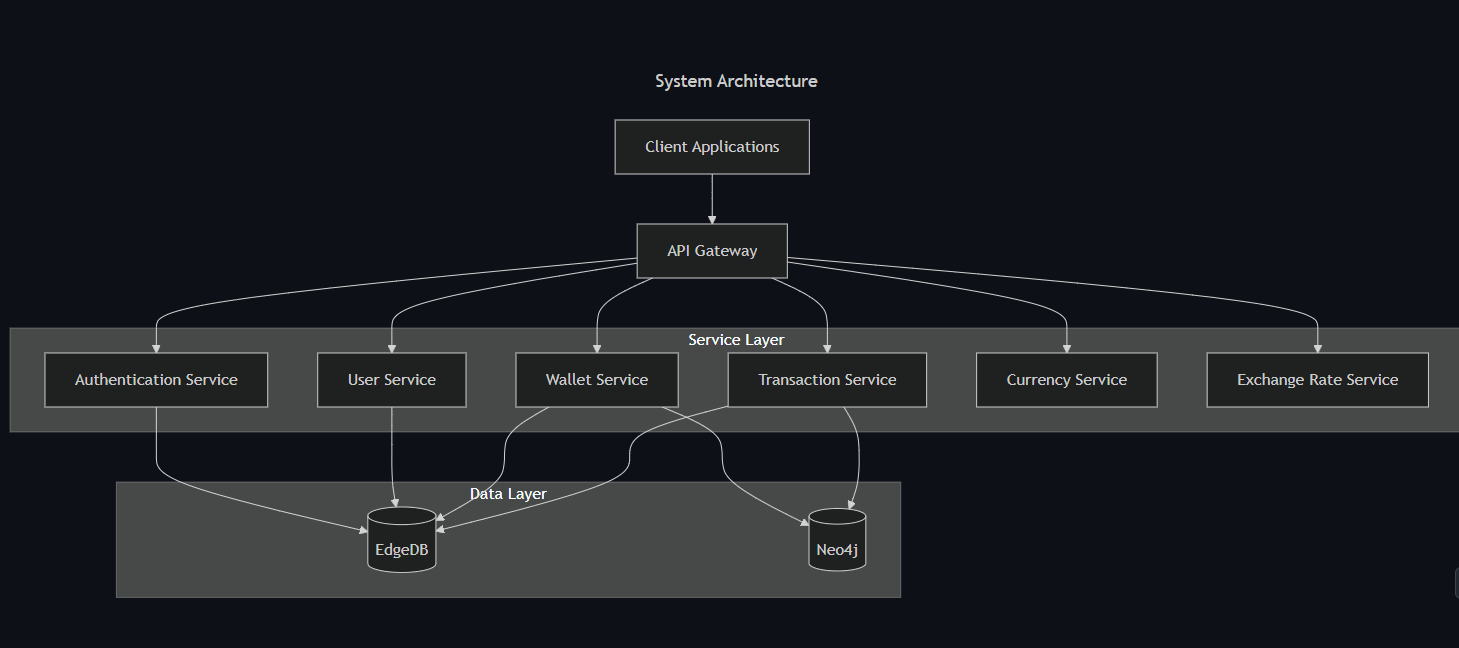
\includegraphics[width=\textwidth, keepaspectratio]{figures/architecture diagram.png}
    \caption{Architecture Diagram}
    \label{fig:Architecture Diagram}
\end{figure}
The architecture (Figure \ref{fig:Architecture Diagram} follows a multi-layered design pattern with clear separation of concerns. It consists of four main layers:

\subsection{Client Layer}
\begin{itemize}
  \item The top layer shows ``Client Applications'' which represent the user-facing interfaces that interact with the system
  \item These applications send requests to the backend services through the API Gateway
\end{itemize}

\subsection{API Gateway Layer}
\begin{itemize}
  \item Serves as the single entry point for all client requests
  \item Handles routing, request aggregation, and potentially authentication/authorization
  \item Directs traffic to the appropriate microservices in the Service Layer below
\end{itemize}

\subsection{Service Layer}
Contains six distinct microservices:
\begin{itemize}
  \item \textbf{Authentication Service}: Manages user identity, login, and security tokens
  \item \textbf{User Service}: Handles user profile management and preferences
  \item \textbf{Wallet Service}: Manages blockchain wallets and associated keys
  \item \textbf{Transaction Service}: Processes blockchain transactions and their metadata
  \item \textbf{Currency Service}: Handles different cryptocurrencies and their specifications
  \item \textbf{Exchange Rate Service}: Provides current and historical exchange rate data
\end{itemize}

\subsection{Data Layer}
Contains two different database systems:
\begin{itemize}
  \item \textbf{EdgeDB}: A graph-relational database that appears to store user, authentication, and possibly wallet data
  \item \textbf{Neo4j}: A graph database that likely stores transaction data, enabling complex relationship queries between transactions
\end{itemize}

\section{Data Flow}
The connections between layers show the flow of data:
\begin{itemize}
  \item Authentication and User services connect to EdgeDB
  \item Wallet and Transaction services connect to both EdgeDB and Neo4j
  \item This dual-database approach suggests different data access patterns for different types of information
\end{itemize}
% system_architecture.tex

\section{Authentication Flow}
\begin{figure}[h]
    \centering
    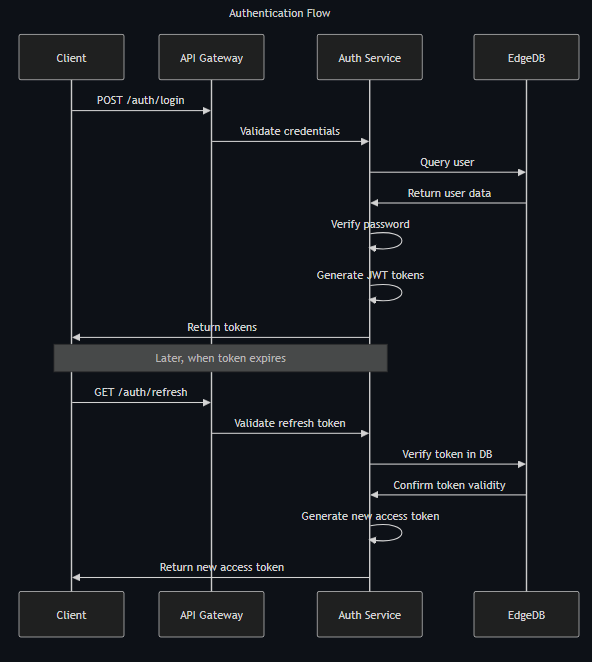
\includegraphics[width=\textwidth, keepaspectratio]{figures/authentication_flow.png}
    \caption{Authentication Flow}
    \label{fig:Authentication Flow}
\end{figure}

The authentication flow diagram (Figure \ref{fig:Authentication Flow}) illustrates a secure, token-based authentication system consisting of four key components: Client, API Gateway, Auth Service, and EdgeDB. The flow is divided into two main processes: initial authentication and token refresh.

\subsection{Initial Authentication Process}

\begin{enumerate}
    \item \textbf{Client Request Initiation}:
    \begin{itemize}
        \item The process begins when the Client sends a POST request to the ``/auth/login'' endpoint of the API Gateway.
        \item This request contains the user's credentials (likely username/email and password).
    \end{itemize}
    
    \item \textbf{Credential Validation}:
    \begin{itemize}
        \item The API Gateway forwards these credentials to the Auth Service for validation.
        \item The Auth Service serves as the central authentication authority in this architecture.
    \end{itemize}
    
    \item \textbf{User Data Retrieval}:
    \begin{itemize}
        \item To validate credentials, the Auth Service queries the EdgeDB database.
        \item EdgeDB returns the user's data, which likely includes the stored password hash and possibly user roles or permissions.
    \end{itemize}
    
    \item \textbf{Password Verification}:
    \begin{itemize}
        \item The Auth Service verifies the provided password against the stored password information.
        \item This likely uses secure hashing techniques to compare passwords without storing them in plaintext.
    \end{itemize}
    
    \item \textbf{JWT Token Generation}:
    \begin{itemize}
        \item Upon successful verification, the Auth Service generates JWT (JSON Web Tokens).
        \item These tokens typically include:
        \begin{itemize}
            \item An access token (short-lived) for API resource access
            \item A refresh token (longer-lived) for obtaining new access tokens
        \end{itemize}
    \end{itemize}
    
    \item \textbf{Token Response}:
    \begin{itemize}
        \item The Auth Service returns these tokens to the Client via the API Gateway.
        \item The Client stores these tokens for subsequent requests to the blockchain visualization system.
    \end{itemize}
\end{enumerate}

\subsection{Token Refresh Process}

\begin{enumerate}
    \item \textbf{Refresh Request}:
    \begin{itemize}
        \item When the access token expires, the Client sends a GET request to ``/auth/refresh''.
        \item This request includes the previously issued refresh token.
    \end{itemize}
    
    \item \textbf{Refresh Token Validation}:
    \begin{itemize}
        \item The API Gateway forwards the refresh token to the Auth Service.
        \item The Auth Service validates the refresh token's integrity and expiration.
    \end{itemize}
    
    \item \textbf{Database Verification}:
    \begin{itemize}
        \item The Auth Service verifies the token against records in EdgeDB.
        \item This step ensures the token hasn't been revoked or invalidated.
    \end{itemize}
    
    \item \textbf{Token Validity Confirmation}:
    \begin{itemize}
        \item EdgeDB confirms the token's validity status back to the Auth Service.
    \end{itemize}
    
    \item \textbf{New Access Token Generation}:
    \begin{itemize}
        \item Upon confirmation, the Auth Service generates a new access token.
        \item This process allows continuous authentication without requiring users to re-enter credentials.
    \end{itemize}
    
    \item \textbf{Token Return}:
    \begin{itemize}
        \item The new access token is returned to the Client via the API Gateway.
        \item The Client can now continue accessing the blockchain transaction visualization system.
    \end{itemize}
\end{enumerate}
This authentication architecture provides a robust security layer for the blockchain transaction information visualization system, ensuring that only authenticated users can access sensitive blockchain data while maintaining a seamless user experience.
\section{Transaction Query Process}
\begin{figure}[h]
    \centering
    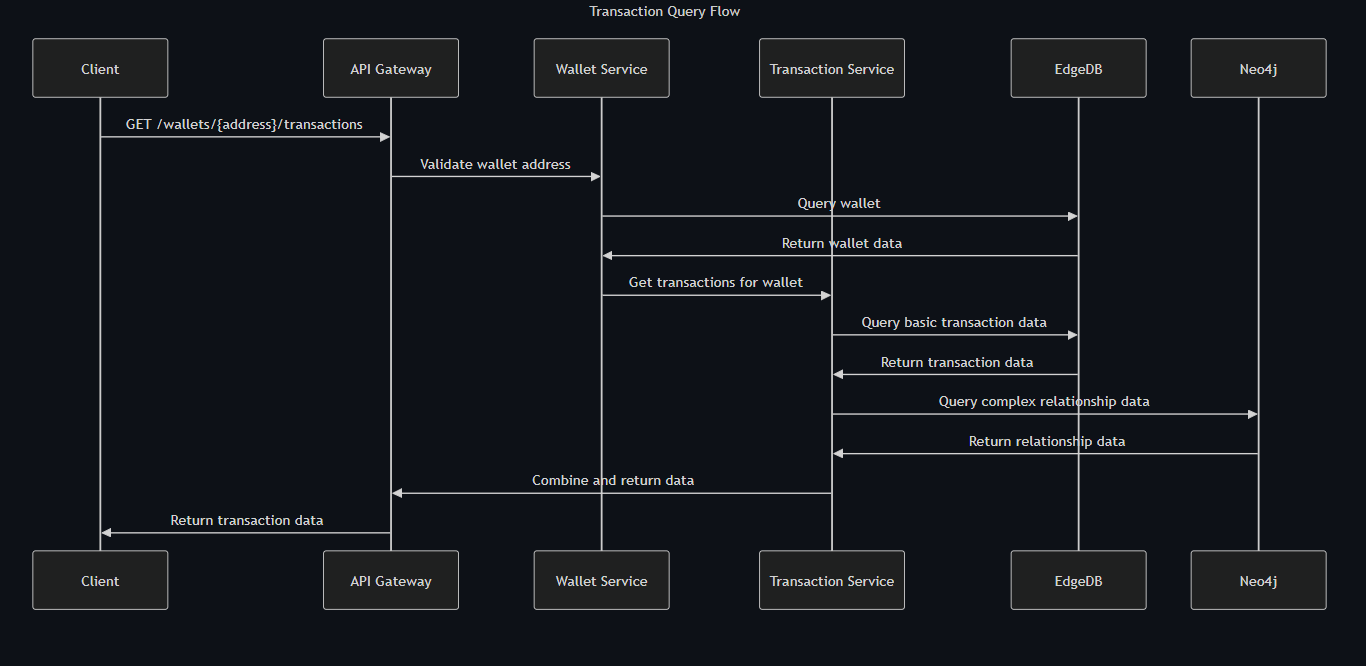
\includegraphics[width=\textwidth, keepaspectratio]{figures/_query.png}
    \caption{Transaction Query}
    \label{fig:Transaction Query}
\end{figure}
This diagram ,see Figure \ref{fig:Transaction Query}, illustrates the comprehensive transaction query process of the blockchain visualization system, showing how transaction data is retrieved and processed through a microservices architecture. The flow involves six key components: Client, API Gateway, Wallet Service, Transaction Service, EdgeDB, and Neo4j:

\begin{enumerate}
    \item \textbf{Client Request Initiation}:
    \begin{itemize}
        \item The flow begins when the Client sends a GET request to ``/wallets/\{address\}/transactions'' through the API Gateway.
        \item This endpoint is designed to retrieve all transactions associated with a specific blockchain wallet address.
    \end{itemize}
    
    \item \textbf{Wallet Address Validation}:
    \begin{itemize}
        \item The API Gateway forwards the request to the Wallet Service.
        \item The Wallet Service performs validation on the provided wallet address to ensure it's correctly formatted and potentially exists in the system.
    \end{itemize}
    
    \item \textbf{Wallet Data Retrieval}:
    \begin{itemize}
        \item The Transaction Service queries EdgeDB to retrieve wallet information.
        \item EdgeDB returns the wallet data, which likely includes wallet metadata, balance information, and wallet status.
    \end{itemize}
    
    \item \textbf{Transaction Retrieval}:
    \begin{itemize}
        \item After confirming the wallet exists, the Transaction Service requests transactions associated with this wallet.
        \item This step involves querying basic transaction data from EdgeDB, which likely stores the fundamental transaction records.
    \end{itemize}
    
    \item \textbf{Basic Transaction Data Return}:
    \begin{itemize}
        \item EdgeDB returns the basic transaction data to the Transaction Service.
        \item This data typically includes transaction hashes, timestamps, values, and basic sender/receiver information.
    \end{itemize}
    
    \item \textbf{Complex Relationship Query}:
    \begin{itemize}
        \item The Transaction Service then queries Neo4j database for complex relationship data.
        \item Neo4j, being a graph database, is particularly suited for handling complex relationships between blockchain entities.
        \item This step retrieves additional contextual information about the transactions, such as:
        \begin{itemize}
            \item Transaction patterns
            \item Connected wallets in the transaction network
            \item Historical relationships between addresses
            \item Potentially suspicious activity patterns
        \end{itemize}
    \end{itemize}
    
    \item \textbf{Relationship Data Return}:
    \begin{itemize}
        \item Neo4j returns the relationship data to the Transaction Service.
        \item This data enriches the basic transaction information with network context.
    \end{itemize}
    
    \item \textbf{Data Aggregation and Processing}:
    \begin{itemize}
        \item The Transaction Service combines the basic transaction data from EdgeDB with the complex relationship data from Neo4j.
        \item This combined dataset provides a comprehensive view of the wallet's transaction history within its network context.
    \end{itemize}
    
    \item \textbf{Final Response}:
    \begin{itemize}
        \item The processed and aggregated data is sent back through the Wallet Service to the API Gateway.
        \item Finally, the API Gateway returns the complete transaction data to the Client.
    \end{itemize}
\end{enumerate}

\section{Key Design Decisions}
\subsection{Dual Database Approach}
\textbf{Decision:} Use both EdgeDB and Neo4j for different aspects of data storage and querying.

\textbf{Rationale:}
\begin{itemize}
\item EdgeDB provides strong typing and schema validation for structured data
\item Neo4j excels at relationship queries needed for transaction graph analysis
\item This combination offers the best of both worlds for cryptocurrency data
\end{itemize}
\subsection{Modular Architecture}
\textbf{Decision:} Organize code into feature modules following NestJS best practices.

\textbf{Rationale:}
\begin{itemize}
\item Improves maintainability by separating concerns
\item Enables independent development of features
\item Facilitates testing and code reuse
\end{itemize}
\subsection{JWT Authentication}
\textbf{Decision:} Use JWT tokens with refresh token rotation for authentication.

\textbf{Rationale:}
\begin{itemize}
\item Stateless authentication reduces database load
\item Refresh tokens enable longer sessions without compromising security
\item Industry standard approach for API authentication
\end{itemize}
\subsection{API Documentation with Swagger}
\textbf{Decision:} Automatically generate API documentation using Swagger.

\textbf{Rationale:}
\begin{itemize}
\item Keeps documentation in sync with code
\item Provides interactive testing interface
\item Improves developer experience
\end{itemize}
\section{Performance Considerations}
\begin{enumerate}
\item \textbf{Database Indexing}: Critical fields like wallet addresses and transaction hashes are indexed for fast lookups.
\item \textbf{Caching Strategy}: Frequently accessed data like exchange rates can be cached to reduce database load.
\item \textbf{Pagination}: All list endpoints support pagination to handle large datasets efficiently.
\item \textbf{Query Optimization}: Complex graph queries are optimized to minimize processing time.
\end{enumerate}
\section{Security Measures}
\begin{enumerate}
    \item \textbf{Authentication}: JWT-based authentication with proper token expiration.
    \item \textbf{Password Handling}: Passwords are hashed using bcrypt before storage.
    \item \textbf{Input Validation}: All inputs are validated using Zod schemas.
    \item \textbf{Rate Limiting}: API endpoints are protected against abuse with rate limiting.
    \item \textbf{CORS Configuration}: Cross-Origin Resource Sharing is properly configured.
\end{enumerate}
\section{Deployment Strategy}
The application is designed to be deployed in a containerized environment using Docker, with separate containers for:
\begin{enumerate}
    \item NestJS API
    \item EdgeDB database
    \item Neo4j database
\end{enumerate}
This enables easy scaling of individual components as needed.

\chapter{Backend Database Design} \label{ch8}
\section{Database Schema Overview}
\paragraph{}The database schema is structured to support a cryptocurrency wallet application with capabilities for tracking transactions, managing multiple currencies, monitoring exchange rates, and providing user account management. The design employs a robust entity-relationship model with appropriate constraints and data types specific to blockchain data requirements.

The database is organized around five primary entities:

\begin{enumerate}
    \item \textbf{Currency} - Represents different cryptocurrencies or tokens
    \item \textbf{ExchangeRate} - Tracks conversion rates between currencies
    \item \textbf{Transaction} - Records blockchain transactions with detailed metadata
    \item \textbf{User} - Manages application users and authentication
    \item \textbf{Wallet} - Represents cryptocurrency wallets owned by users
\end{enumerate}

Each entity inherits from a common BaseObject type, ensuring consistent handling of identifiers and providing a foundation for entity relationships.
\newpage
\begin{figure}[H]
    \centering
    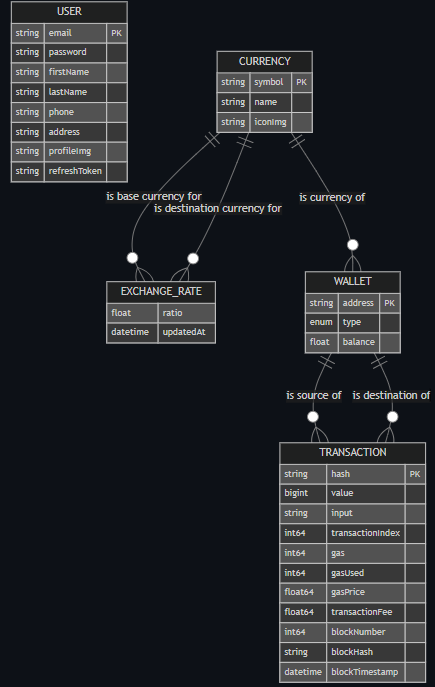
\includegraphics[width= 1\textwidth]{figures/ERD diagram.png}
     \caption{ERD of Database}
    \label{fig:ERD}
\end{figure}
\section{Crypto Exchange Platform Data Models}
% User Model Table
\begin{table}[htbp]
  \centering
  \caption{User}
  \footnotesize
  \renewcommand{\arraystretch}{1.4}
  \setlength{\tabcolsep}{6pt}
  \begin{tabular}{|l|l|c|p{4cm}|p{2.8cm}|}
    \hline
    \textbf{Field} & \textbf{Type} & \textbf{Required} & \textbf{Description} & \textbf{Constraints} \\
    \hline
    email & String & Yes & User email address & Unique \\
    \hline
    normalizedEmail & String & No & Normalized version of email & Unique \\
    \hline
    password & String & Yes & Hashed password & \\
    \hline
    firstName & String & No & User's first name & \\
    \hline
    lastName & String & No & User's last name & \\
    \hline
    fullName & String & No & Computed full name & Computed field \\
    \hline
    phone & String & No & User's phone number & \\
    \hline
    address & String & No & User's physical address & \\
    \hline
    profileImg & String & No & URL to profile image & \\
    \hline
    refreshToken & String & No & Token for authentication refresh & \\
    \hline
  \end{tabular}
\end{table}

% Currency Model Table
\begin{table}[htbp]
  \centering
  \caption{Currency}
  \footnotesize
  \renewcommand{\arraystretch}{1.1}
  \setlength{\tabcolsep}{6pt}
  \begin{tabular}{|l|l|c|p{4cm}|p{2.8cm}|}
    \hline
    \textbf{Field} & \textbf{Type} & \textbf{Required} & \textbf{Description} & \textbf{Constraints} \\
    \hline
    symbol & String & Yes & Currency symbol (e.g., ETH) & Unique \\
    \hline
    name & String & Yes & Full name (e.g., Ethereum) & Unique \\
    \hline
    iconImg & String & Yes & URL to currency icon image & \\
    \hline
  \end{tabular}
\end{table}

% ExchangeRate Model Table
\begin{table}[htbp]
  \centering
  \caption{ExchangeRate}
  \footnotesize
  \renewcommand{\arraystretch}{1.1}
  \setlength{\tabcolsep}{6pt}
  \begin{tabular}{|l|l|c|p{4cm}|p{2.8cm}|}
    \hline
    \textbf{Field} & \textbf{Type} & \textbf{Required} & \textbf{Description} & \textbf{Constraints} \\
    \hline
    ratio & Float64 & Yes & Exchange ratio between currencies & \\
    \hline
    baseCurrency & Currency & Yes & Source currency & Foreign Key \\
    \hline
    destinationCurrency & Currency & Yes & Target currency & Foreign Key \\
    \hline
    updatedAt & DateTime & Yes & Last update timestamp & \\
    \hline
  \end{tabular}
\end{table}

% Wallet Model Table
\begin{table}[htbp]
  \centering
  \caption{Wallet}
  \footnotesize
  \renewcommand{\arraystretch}{1.1}
  \setlength{\tabcolsep}{6pt}
  \begin{tabular}{|l|l|c|p{4cm}|p{2.8cm}|}
    \hline
    \textbf{Field} & \textbf{Type} & \textbf{Required} & \textbf{Description} & \textbf{Constraints} \\
    \hline
    address & String & Yes & Wallet address & Unique \\
    \hline
    type & WalletType & Yes & EOA or Contract & Enum \\
    \hline
    balance & Float64 & Yes & Current balance & Default: 0.0 \\
    \hline
    currency & Currency & Yes & Currency of the wallet & Foreign Key \\
    \hline
  \end{tabular}
\end{table}

% Transaction Model Table
\begin{table}[htbp]
  \centering
  \caption{Transaction}
  \footnotesize
  \renewcommand{\arraystretch}{1.1}
  \setlength{\tabcolsep}{6pt}
  \begin{tabular}{|l|l|c|p{4cm}|p{2.8cm}|}
    \hline
    \textbf{Field} & \textbf{Type} & \textbf{Required} & \textbf{Description} & \textbf{Constraints} \\
    \hline
    hash & String & Yes & Transaction hash & Unique \\
    \hline
    value & BigInt & Yes & Transaction amount & \\
    \hline
    sourceWallet & Wallet & Yes & Source wallet & Foreign Key \\
    \hline
    destinationWallet & Wallet & Yes & Destination wallet & Foreign Key \\
    \hline
    input & String & Yes & Transaction input data & \\
    \hline
    transactionIndex & Int64 & Yes & Index in the block & \\
    \hline
    gas & Int64 & Yes & Gas limit & \\
    \hline
    gasUsed & Int64 & Yes & Gas used & \\
    \hline
    gasPrice & Float64 & Yes & Gas price & \\
    \hline
    transactionFee & Float64 & Yes & Total transaction fee & \\
    \hline
    blockNumber & Int64 & Yes & Block number & \\
    \hline
    blockHash & String & Yes & Block hash & \\
    \hline
    blockTimestamp & DateTime & Yes & Block timestamp & \\
    \hline
  \end{tabular}
\end{table}

% Relationships Table
\begin{table}[htbp]
  \centering
  \caption{Relationships}
  \footnotesize
  \renewcommand{\arraystretch}{1.4}
  \setlength{\tabcolsep}{6pt}
  \begin{tabular}{|l|l|p{7cm}|}
    \hline
    \textbf{Relationship} & \textbf{Type} & \textbf{Description} \\
    \hline
    Currency $\rightarrow$ ExchangeRate & One-to-Many & A currency can be the base for many exchange rates \\
    \hline
    Currency $\rightarrow$ ExchangeRate & One-to-Many & A currency can be the destination for many rates \\
    \hline
    Currency $\rightarrow$ Wallet & One-to-Many & A currency can have many wallets \\
    \hline
    Wallet $\rightarrow$ Transaction (source) & One-to-Many & A wallet can be the source of many transactions \\
    \hline
    Wallet $\rightarrow$ Transaction (dest) & One-to-Many & A wallet can be the destination of many transactions \\
    \hline
  \end{tabular}
\end{table}

% Indexes Table
\begin{table}[htbp]
  \centering
  \caption{Indexes}
  \footnotesize
  \renewcommand{\arraystretch}{1.4}
  \setlength{\tabcolsep}{6pt}
  \begin{tabular}{|l|l|l|p{4.8cm}|}
    \hline
    \textbf{Model} & \textbf{Fields} & \textbf{Type} & \textbf{Description} \\
    \hline
    User & email & Unique & Fast lookup by email \\
    \hline
    Currency & symbol & Unique & Fast lookup by currency symbol \\
    \hline
    Currency & name & Unique & Fast lookup by currency name \\
    \hline
    Wallet & address & Unique & Fast lookup by wallet address \\
    \hline
    Transaction & hash & Unique & Fast lookup by transaction hash \\
    \hline
  \end{tabular}
\end{table}

\begin{table}[htbp]
  \centering
  \caption{Constraints and Validations}
  \footnotesize
  \renewcommand{\arraystretch}{1.4}
  \setlength{\tabcolsep}{6pt}
  \begin{tabular}{|l|l|l|p{5cm}|}
    \hline
    \textbf{Model} & \textbf{Field} & \textbf{Validation} & \textbf{Description} \\
    \hline
    User & email & Exclusive & Email must be unique \\
    \hline
    User & normalizedEmail & Exclusive & Normalized email must be unique \\
    \hline
    Currency & symbol & Exclusive & Currency symbol must be unique \\
    \hline
    Currency & name & Exclusive & Currency name must be unique \\
    \hline
    Wallet & address & Exclusive & Wallet address must be unique \\
    \hline
    Wallet & type & Enum & Must be either EOA or Contract \\
    \hline
    Transaction & hash & Exclusive & Transaction hash must be unique \\
    \hline
  \end{tabular}
\end{table}
\subsection{Example Usage}
\begin{tcolorbox}[width=\textwidth, boxrule=0.5pt, colback=gray!5, colframe=gray!50]
\begin{minted}[fontsize=\small, breaklines=true]{javascript}
// Get a user by email
const user = await e.select(e.User, (user) => ({
  filter_single: { email: 'user@example.com' },
}));

// Get all wallets for a specific currency
const ethWallets = await e.select(e.Wallet, (wallet) => ({
  filter: e.op(wallet.currency.symbol, '=', 'ETH'),
}));

// Get exchange rate between two currencies
const ethToBtcRate = await e.select(e.ExchangeRate, (rate) => ({
  filter_single: {
    baseCurrency: { symbol: 'ETH' },
    destinationCurrency: { symbol: 'BTC' },
  },
}));

// Get all transactions from a specific wallet
const transactions = await e.select(e.Transaction, (tx) => ({
  filter: e.op(tx.sourceWallet.address, '=', '0x123...'),
}));
\end{minted}
\end{tcolorbox}
\section*{Notes and Considerations}

\begin{itemize}
  \item The system uses EdgeDB as the primary database
  \item Wallet balances are stored as float64 which may not be ideal for financial calculations - consider using a fixed-point representation or string-based storage for production
  \item Transaction values are stored as bigint to handle large cryptocurrency amounts
  \item The system currently doesn't have explicit user-wallet ownership relationships - consider adding this if needed
  \item Exchange rates should be regularly updated from external sources
\end{itemize}
\section{User and Cryptocurrency Data Models}
\subsection{Overview}
Core data models for user management, cryptocurrency wallets, transactions, and exchange rates in the COS30049 Blockchain-based Cryptocurrency Exchange platform.
\subsection{Data Models}
\begin{table}[htbp]
  \centering
  \caption{User}
  \renewcommand{\arraystretch}{1.5}
  \begin{tabular}{|p{3cm}|p{2cm}|c|p{4cm}|p{4cm}|}
    \hline
    \textbf{Field} & \textbf{Type} & \textbf{Required} & \textbf{Description} & \textbf{Constraints} \\
    \hline
    email & string & Yes & User email address & Primary Key, Unique \\
    \hline
    normalizedEmail & string & No & Normalized email for case-insensitive lookups & Unique \\
    \hline
    password & string & Yes & Hashed password & \\
    \hline
    firstName & string & No & User's first name & \\
    \hline
    lastName & string & No & User's last name & \\
    \hline
    fullName & string & No & Computed full name & Computed from firstName + lastName \\
    \hline
    phone & string & No & User's phone number & \\
    \hline
    address & string & No & User's physical address & \\
    \hline
    profileImg & string & No & URL to user's profile image & \\
    \hline
    refreshToken & string & No & JWT refresh token & \\
    \hline
  \end{tabular}
\end{table}

\begin{table}[htbp]
  \centering
  \caption{Currency}
  \renewcommand{\arraystretch}{1.5}
  \begin{tabular}{|p{3cm}|p{2cm}|c|p{4cm}|p{4cm}|}
    \hline
    \textbf{Field} & \textbf{Type} & \textbf{Required} & \textbf{Description} & \textbf{Constraints} \\
    \hline
    symbol & string & Yes & Currency symbol (e.g., ETH) & Primary Key, Unique \\
    \hline
    name & string & Yes & Full name (e.g., Ethereum) & Unique \\
    \hline
    iconImg & string & Yes & URL to currency icon image & \\
    \hline
  \end{tabular}
\end{table}

\begin{table}[htbp]
  \centering
  \caption{ExchangeRate}
  \renewcommand{\arraystretch}{1.5}
  \begin{tabular}{|p{3cm}|p{2cm}|c|p{4cm}|p{4cm}|}
    \hline
    \textbf{Field} & \textbf{Type} & \textbf{Required} & \textbf{Description} & \textbf{Constraints} \\
    \hline
    ratio & float64 & Yes & Exchange rate ratio & \\
    \hline
    baseCurrency & Currency & Yes & Reference to base currency & Foreign Key \\
    \hline
    destinationCurrency & Currency & Yes & Reference to destination currency & Foreign Key \\
    \hline
    updatedAt & datetime & Yes & Last update timestamp & \\
    \hline
  \end{tabular}
\end{table}

\begin{table}[htbp]
  \centering
  \caption{Wallet}
  \renewcommand{\arraystretch}{1.5}
  \begin{tabular}{|p{3cm}|p{2cm}|c|p{4cm}|p{4cm}|}
    \hline
    \textbf{Field} & \textbf{Type} & \textbf{Required} & \textbf{Description} & \textbf{Constraints} \\
    \hline
    address & string & Yes & Wallet address & Primary Key, Unique \\
    \hline
    type & enum & Yes & Wallet type (EOA or Contract) & \\
    \hline
    balance & float64 & Yes & Current balance & Default: 0.0 \\
    \hline
    currency & Currency & Yes & Reference to currency & Foreign Key \\
    \hline
  \end{tabular}
\end{table}

\begin{table}[htbp]
  \centering
  \caption{Transaction}
  \renewcommand{\arraystretch}{1.5}
  \begin{tabular}{|p{3cm}|p{2cm}|c|p{4cm}|p{4cm}|}
    \hline
    \textbf{Field} & \textbf{Type} & \textbf{Required} & \textbf{Description} & \textbf{Constraints} \\
    \hline
    hash & string & Yes & Transaction hash & Primary Key, Unique \\
    \hline
    value & bigint & Yes & Transaction amount & \\
    \hline
    sourceWallet & Wallet & Yes & Reference to source wallet & Foreign Key \\
    \hline
    destinationWallet & Wallet & Yes & Reference to destination wallet & Foreign Key \\
    \hline
    input & string & Yes & Transaction input data & \\
    \hline
    transactionIndex & int64 & Yes & Index in the block & \\
    \hline
    gas & int64 & Yes & Gas limit & \\
    \hline
    gasUsed & int64 & Yes & Gas used & \\
    \hline
    gasPrice & float64 & Yes & Gas price & \\
    \hline
    transactionFee & float64 & Yes & Total transaction fee & \\
    \hline
    blockNumber & int64 & Yes & Block number & \\
    \hline
    blockHash & string & Yes & Block hash & \\
    \hline
    blockTimestamp & datetime & Yes & Block timestamp & \\
    \hline
  \end{tabular}
\end{table}

\begin{table}[htbp]
  \centering
  \caption{Relationships}
  \renewcommand{\arraystretch}{1.5}
  \begin{tabular}{|p{5.5cm}|p{3cm}|p{6cm}|}
    \hline
    \textbf{Relationship} & \textbf{Type} & \textbf{Description} \\
    \hline
    User$\rightarrow$Wallet & One-to-Many & A user can own multiple wallets \\
    \hline
    Currency$\rightarrow$Wallet & One-to-Many & A currency can be used by multiple wallets \\
    \hline
    Currency$\rightarrow$ExchangeRate (base) & One-to-Many & A currency can be the base in multiple exchange rates \\
    \hline
    Currency$\rightarrow$ExchangeRate (destination) & One-to-Many & A currency can be the destination in multiple exchange rates \\
    \hline
    Wallet$\rightarrow$Transaction (source) & One-to-Many & A wallet can be the source of multiple transactions \\
    \hline
    Wallet$\rightarrow$Transaction (destination) & One-to-Many & A wallet can be the destination of multiple transactions \\
    \hline
  \end{tabular}
\end{table}

\begin{table}[htbp]
  \centering
  \caption{Indexes}
  \renewcommand{\arraystretch}{1.5}
  \begin{tabular}{|p{3cm}|p{3cm}|p{3cm}|p{6cm}|}
    \hline
    \textbf{Model} & \textbf{Fields} & \textbf{Type} & \textbf{Description} \\
    \hline
    User & email & Unique & Fast lookup by email \\
    \hline
    User & normalizedEmail & Unique & Case-insensitive email lookup \\
    \hline
    Currency & symbol & Unique & Fast lookup by symbol \\
    \hline
    Currency & name & Unique & Fast lookup by name \\
    \hline
    Wallet & address & Unique & Fast lookup by wallet address \\
    \hline
    Transaction & hash & Unique & Fast lookup by transaction hash \\
    \hline
  \end{tabular}
\end{table}

\begin{table}[htbp]
  \centering
  \caption{Constraints and Validations}
  \renewcommand{\arraystretch}{1.5}
  \begin{tabular}{|p{3cm}|p{4.5cm}|p{7cm}|}
    \hline
    \textbf{Model} & \textbf{Constraint} & \textbf{Description} \\
    \hline
    User & Email format & Email must be in valid format \\
    \hline
    User & Password complexity & Password must meet complexity requirements \\
    \hline
    Currency & Symbol format & Symbol must be uppercase letters \\
    \hline
    Wallet & Address format & Address must be valid blockchain address \\
    \hline
    Transaction & Positive value & Transaction value must be positive \\
    \hline
    Transaction & Source != Destination & Source and destination wallets must differ \\
    \hline
  \end{tabular}
\end{table}
\subsection{Example Use}
\subsubsection*{Creating a User}
\begin{tcolorbox}[width=\textwidth, boxrule=0.5pt, colback=gray!5, colframe=gray!50]
\begin{minted}[fontsize=\small, breaklines=true]{javascript}
const user = await e.insert(e.User, {
  email: 'user@example.com',
  normalizedEmail: 'user@example.com'.toLowerCase(),
  password: await bcrypt.hash('securePassword123', 10),
  firstName: 'John',
  lastName: 'Doe',
  phone: '+1234567890',
  address: '123 Main St, City, Country',
});
\end{minted}
\end{tcolorbox}
\subsubsection*{Creating a Wallet}
\begin{tcolorbox}[width=\textwidth, boxrule=0.5pt, colback=gray!5, colframe=gray!50]
\begin{minted}[fontsize=\small, breaklines=true]{javascript}
const currency = await e.select(e.Currency, (c) => ({
  filter: e.op(c.symbol, '=', 'ETH'),
}));

const wallet = await e.insert(e.Wallet, {
  address: '0x742d35Cc6634C0532925a3b844Bc454e4438f44e',
  type: 'EOA',
  balance: 1.25,
  currency: currency,
});
\end{minted}
\end{tcolorbox}
\subsubsection*{Querying Transactions}
\begin{tcolorbox}[width=\textwidth, boxrule=0.5pt, colback=gray!5, colframe=gray!50]
\begin{minted}[fontsize=\small, breaklines=true]{javascript}
const transactions = await e.select(e.Transaction, (t) => ({
  filter: e.op(
    t.sourceWallet.address,
    '=',
    '0x742d35Cc6634C0532925a3b844Bc454e4438f44e',
  ),
  order_by: {
    expression: t.blockTimestamp,
    direction: e.DESC,
  },
  limit: 10,
}));
\end{minted}
\end{tcolorbox}


\chapter{API Documentation} \label{ch9}
\section{Technical Summary}
This API provides a comprehensive backend for a blockchain-based cryptocurrency exchange platform. It enables users to manage wallets, view transactions, authenticate, and interact with cryptocurrency data. The system is built on a modern architecture using NestJS and EdgeDB, with additional graph database capabilities through Neo4j for complex relationship queries.
\begin{table}[htbp]
\centering
\renewcommand{\arraystretch}{1.3}
\setlength{\tabcolsep}{12pt}
\begin{tabular}{|l|p{0.75\textwidth}|}
\hline
\textbf{Technology} & \textbf{Description} \\
\hline
NestJS & Progressive Node.js framework for building server-side applications \\
\hline
EdgeDB & Next-generation graph-relational database \\
\hline
Neo4j & Graph database for complex relationship queries \\
\hline
JWT & JSON Web Tokens for secure authentication \\
\hline
Swagger & API documentation and testing \\
\hline
TypeScript & Typed JavaScript for better developer experience \\
\hline
Zod & Schema validation library \\
\hline
Pino & Logging library \\
\hline
\end{tabular}
\caption{Technology Table}
\end{table}

\newpage
\section{API Architecture Diagram}
\begin{figure}[h]
    \centering
    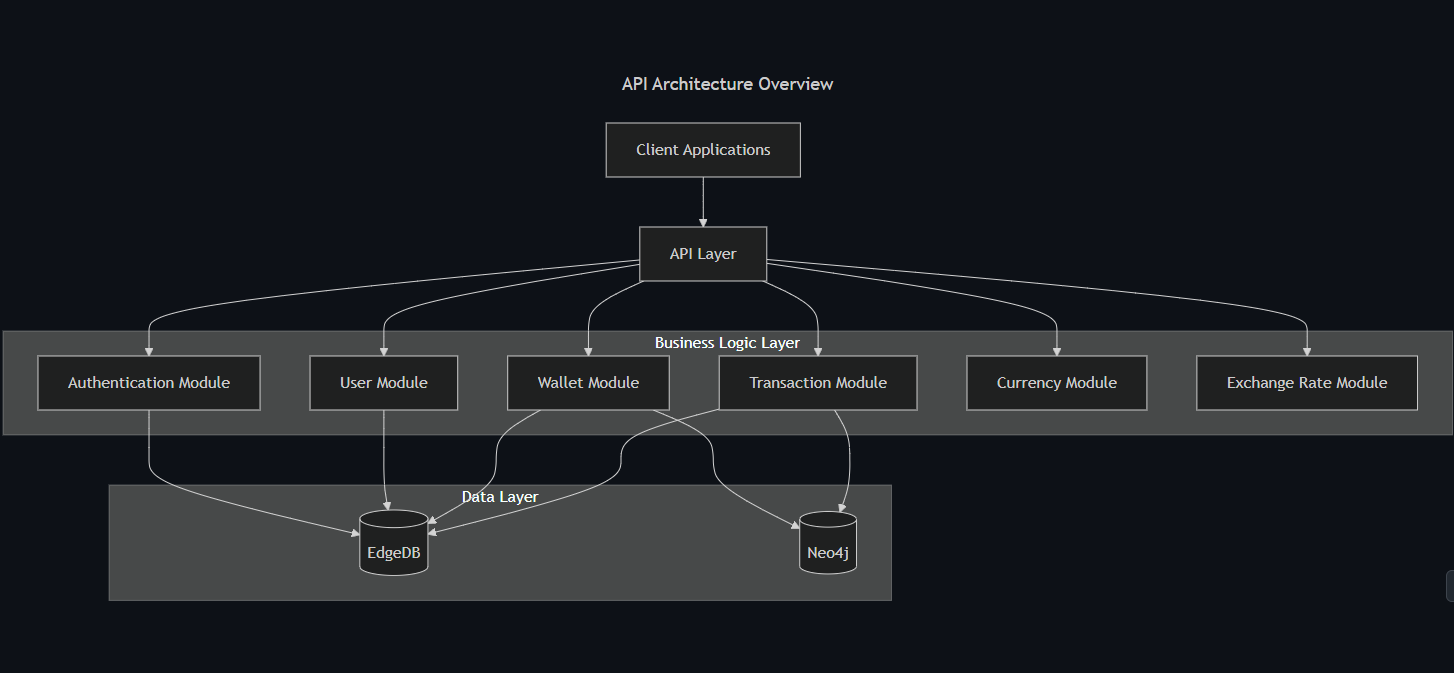
\includegraphics[width=\textwidth, keepaspectratio]{figures/api_architecture.png}
    \caption{API Architecture}
    \label{fig:api_architecture}
\end{figure}

The architecture diagram, see Figure \ref{fig:api_architecture}, illustrates a comprehensive blockchain transaction visualization system designed with a multi-layered approach:
The \textbf{Client Applications} layer serves as the user-facing interface where stakeholders interact with the blockchain data visualization tools.
The \textbf{API Layer} acts as the centralized gateway, coordinating requests and responses between client applications and the underlying business logic.
The Business Logic Layer comprises six specialized modules:
\begin{itemize}
\item \textbf{Authentication Module:} Secures access through blockchain-specific identity verification
\item \textbf{User Module:} Manages user profiles and permissions for blockchain data access
\item \textbf{Wallet Module:} Connects to and monitors blockchain wallet addresses
\item \textbf{Transaction Module:} Processes and analyzes blockchain transaction data
\item \textbf{Currency Module:} Tracks various cryptocurrencies and tokens
\item \textbf{Exchange Rate Module:} Monitors real-time cryptocurrency valuations
\end{itemize}
The Data Layer leverages two complementary database technologies:
\begin{itemize}
\item \textbf{EdgeDB:} Stores structured blockchain data, user information, and authentication details
\item \textbf{Neo4j:} Graph database optimized for blockchain transaction relationship mapping and visualization
\end{itemize}

\section{API Endpoints}

\subsection*{Authentication}
\renewcommand{\arraystretch}{1.5}
\begin{tabular}{|p{0.28\textwidth}|p{0.18\textwidth}|p{0.54\textwidth}|}
\hline
\textbf{Endpoint} & \textbf{Method} & \textbf{Description} \\
\hline
/auth/login & POST & Authenticate user and receive JWT tokens \\
\hline
/auth/refresh & GET & Refresh access token using refresh token \\
\hline
\end{tabular}

\subsection*{Users}
\renewcommand{\arraystretch}{1.5}
\begin{tabular}{|p{0.28\textwidth}|p{0.18\textwidth}|p{0.54\textwidth}|}
\hline
\textbf{Endpoint} & \textbf{Method} & \textbf{Description} \\
\hline
/users & POST & Create a new user account \\
\hline
\end{tabular}

\subsection*{Wallets}
\renewcommand{\arraystretch}{1.5}
\begin{tabular}{|p{0.38\textwidth}|p{0.12\textwidth}|p{0.5\textwidth}|}
\hline
\textbf{Endpoint} & \textbf{Method} & \textbf{Description} \\
\hline
/wallets & GET & Get all wallets with optional filtering \\
\hline
/wallets/:address & GET & Get wallet details by address \\
\hline
/wallets/:address/details & GET & Get detailed wallet information \\
\hline
/wallets/:address/transactions & GET & Get transactions for a specific wallet \\
\hline
/wallets/:address/neighbors & GET & Get wallets that have transactions with the specified wallet \\
\hline
\end{tabular}

\subsection*{Transactions}
\renewcommand{\arraystretch}{1.5}
\begin{tabular}{|p{0.38\textwidth}|p{0.12\textwidth}|p{0.5\textwidth}|}
\hline
\textbf{Endpoint} & \textbf{Method} & \textbf{Description} \\
\hline
/transactions/graph & GET & Get transaction graph data for visualization \\
\hline
\end{tabular}

\section{Request and Response Examples}
% Using boxed environment instead of black background

\subsection*{Authentication}

\subsubsection*{Login}

\textbf{Request:}

\begin{tcolorbox}[width=\textwidth, boxrule=0.5pt, colback=gray!5, colframe=gray!50]
\begin{minted}[breaklines]{bash}
POST /users
Content-Type: application/json
\end{minted}

\begin{minted}{json}
{
  "email": "user@example.com",
  "password": "securePassword123"
}
\end{minted}
\end{tcolorbox}

\vspace{1em}
\textbf{Response:}

\begin{tcolorbox}[width=\textwidth, boxrule=0.5pt, colback=gray!5, colframe=gray!50]
\begin{minted}[breaklines]{json}
{
  "accessToken": "eyJhbGciOiJIUzI1NiIsInR5cCI6IkpXVCJ9...",
  "refreshToken": "eyJhbGciOiJIUzI1NiIsInR5cCI6IkpXVCJ9..."
}
\end{minted}
\end{tcolorbox}

\subsection*{Users}

\subsubsection*{Create User}

\textbf{Request:}

\begin{tcolorbox}[width=\textwidth, boxrule=0.5pt, colback=gray!5, colframe=gray!50]
\begin{minted}[breaklines]{bash}
POST /users
Content-Type: application/json
\end{minted}

\begin{minted}[breaklines]{json}
{
  "email": "newuser@example.com",
  "password": "securePassword123",
  "firstName": "John",
  "lastName": "Doe"
}
\end{minted}
\end{tcolorbox}

\vspace{1em}
\textbf{Response:}

\begin{tcolorbox}[width=\textwidth, boxrule=0.5pt, colback=gray!5, colframe=gray!50]
\begin{minted}{json}
{
  "id": "123e4567-e89b-12d3-a456-426614174000",
  "email": "newuser@example.com",
  "firstName": "John",
  "lastName": "Doe",
  "fullName": "John Doe"
}
\end{minted}
\end{tcolorbox}

\subsection*{Wallets}

\subsubsection*{Get Wallet Details}

\textbf{Request:}

\begin{tcolorbox}[width=\textwidth, boxrule=0.5pt, colback=gray!5, colframe=gray!50]
\begin{minted}[breaklines, breakanywhere]{bash}
GET /wallets/0x742d35cc6634c0532925a3b844bc454e4438f44e/details
\end{minted}
\end{tcolorbox}

\vspace{1em}
\textbf{Response:}

\begin{tcolorbox}[width=\textwidth, boxrule=0.5pt, colback=gray!5, colframe=gray!50]
\begin{minted}{json}
{
  "address": "0x742d35cc6634c0532925a3b844bc454e4438f44e",
  "type": "EOA",
  "balance": 1.25,
  "currency": {
    "symbol": "ETH",
    "name": "Ethereum",
    "iconImg": "https://example.com/eth-icon.png"
  },
  "transactionCount": 42,
  "incomingTransactionCount": 15,
  "outgoingTransactionCount": 27
}
\end{minted}
\end{tcolorbox}

\subsection*{Get Wallet Transactions}

\textbf{Request:}

\begin{tcolorbox}[width=\textwidth, boxrule=0.5pt, colback=gray!5, colframe=gray!50]
\begin{minted}[
    breaklines=true,
    breakanywhere=true,
]{bash}
GET /wallets/0x742d35cc6634c0532925a3b844bc454e4438f44e/transactions?type=INCOMING
\end{minted}
\end{tcolorbox}


\vspace{1em}
\textbf{Response:}

\begin{tcolorbox}[width=\textwidth, boxrule=0.5pt, colback=gray!5, colframe=gray!50]
\begin{minted}[breaklines, breakanywhere=true, escapeinside=||]{json}
{
  "transactions": [
    {
      "hash": "0x1234567890abcdef1234567890abcdef1234567890abcdef",
      "value": "1000000000000000000",
      "sourceWallet": {
        "address": "0x11111222233334444555566667777888899999aaaa"
      },
      "destinationWallet": {
        "address": "0x742d35cc6634c0532925a3b844bc454e4438f44e"
      },
      "blockTimestamp": "2023-01-15T12:30:45Z",
      "transactionFee": 0.002
    }
    |\textcolor{gray}{// More transactions...}|
  ],
  "total": 15
}
\end{minted}
\end{tcolorbox}
\section{Error Handling}
The API uses standard HTTP status codes to indicate the success or failure of requests:
\begin{table}[htbp]
\centering
\renewcommand{\arraystretch}{1.3}
\setlength{\tabcolsep}{12pt}
\begin{tabular}{|l|p{0.75\textwidth}|}
\hline
\textbf{Status Code} & \textbf{Description} \\
\hline
200 & OK - The request was successful \\
\hline
201 & Created - A new resource was successfully created \\
\hline
400 & Bad Request - The request was invalid or cannot be served \\
\hline
401 & Unauthorized - Authentication is required and has failed or not been provided \\
\hline
403 & Forbidden - The server understood the request but refuses to authorize it \\
\hline
404 & Not Found - The requested resource could not be found \\
\hline
500 & Internal Server Error - An error occurred on the server \\
\hline

\end{tabular}
\caption{Status code}
\end{table}

Error responses follow this format:
\begin{tcolorbox}[width=\textwidth, boxrule=0.5pt, colback=gray!5, colframe=gray!50]
\begin{minted}[breaklines, breakanywhere=true, escapeinside=||]{json}
{
  {
  "statusCode": 400,
  "message": "Validation failed",
  "error": "Bad Request",
  "details": [
    {
      "field": "email",
      "message": "Invalid email format"
    }
  ]
}
}
\end{minted}
\end{tcolorbox}
\section{Authentication}
The API uses JWT (JSON Web Tokens) for authentication. To access protected endpoints:
\begin{enumerate}
    \item Obtain an access token by logging in via /auth/login
    \item Include the token in the Authorization header of subsequent requests:
    \begin{tcolorbox}[width=\textwidth, boxrule=0.5pt, colback=gray!5, colframe=gray!50]
\begin{minted}[
    breaklines=true,
    breakanywhere=true,
]{bash}
Authorization: Bearer <your_access_token>
\end{minted}
\end{tcolorbox}
    \item When the access token expires, use the refresh token at /auth/refresh to obtain a new access token
\begin{tcolorbox}[width=\textwidth, boxrule=0.5pt, colback=gray!5, colframe=gray!50]
\small % Adjust font size (you can also try \footnotesize or \scriptsize)
\textbf{\textcolor{red}{Warning:}} Never share your JWT tokens or store them in insecure locations.

\end{tcolorbox}
\end{enumerate}
\section{Rate Limiting}

To ensure service stability, the API implements rate limiting:
\begin{itemize}
    \item 100 requests per minute for authenticated users
    \item 20 requests per minute for unauthenticated users
\end{itemize}
\begin{tcolorbox}[width=\textwidth, boxrule=0.5pt, colback=gray!5, colframe=gray!50]
\small % Adjust font size (you can also try \footnotesize or \scriptsize)
\textbf{\textcolor{blue}{Note:}} Rate limit information is included in response headers:
\begin{itemize}
    \item \texttt{X-RateLimit-Limit}: Maximum requests allowed in the time window
    \item \texttt{X-RateLimit-Remaining}: Remaining requests in the current window
    \item \texttt{X-RateLimit-Reset}: Time when the rate limit window resets (Unix timestamp)
\end{itemize}
\end{tcolorbox}
\section{Versioning}
The API uses URL versioning. The current version is v1, which is included in the base URL:
  \begin{tcolorbox}[width=\textwidth, boxrule=0.5pt, colback=gray!5, colframe=gray!50]
\begin{minted}[
    breaklines=true,
    breakanywhere=true,
]{bash}
/api/v1/
\end{minted}
\end{tcolorbox}
\section{Getting Started}

 To start using the API:

\begin{enumerate}
  \item Register a user account via \colorbox{yellow!30}{\texttt{/users}}
  \item Authenticate via \colorbox{yellow!30}{\texttt{/auth/login}}
  \item Use the returned JWT token in the Authorization header for subsequent requests
  \item Explore wallet and transaction data using the provided endpoints
\end{enumerate}
\section{Development and Testing}
The API includes Swagger documentation accessible at  \colorbox{yellow!30}{\texttt{/api/docs}} when running in development mode.

\chapter{Function Description} \label{ch10}
\input{sources/10_function_des}

\chapter{Deployment Instruction} \label{ch11}
\section{Front-end Deployment Guide}
This is a \href{https://nextjs.org/}{\colorbox{yellow!30}{\texttt{Next.js }}}project bootstrapped with\href{https://nextjs.org/docs/app/api-reference/cli/create-next-app}{\colorbox{yellow!30}{\texttt{create-next-app}}} 
\subsection*{Getting Started}
\begin{itemize}

  \item First, install the dependencies:
  \begin{tcolorbox}[width=\textwidth, boxrule=0.5pt, colback=gray!5, colframe=gray!50]
\begin{minted}[
    breaklines=true,
    breakanywhere=true,
]{bash}
pnpm install
\end{minted}
\end{tcolorbox}
  \item Run the development server:
  \begin{tcolorbox}[width=\textwidth, boxrule=0.5pt, colback=gray!5, colframe=gray!50]
\begin{minted}[
    breaklines=true,
    breakanywhere=true,
]{bash}
pnpm run dev
\end{minted}
\end{tcolorbox}
   \end{itemize}
\subsection*{Note:}

The .env with the links to the backend is already included in the zip file (submission),  so it should connect.

The backend may take \textasciitilde{}1 minute to boot up from sleep since we are on the Free tier of the hosting platform. As such, please wait for the results (especially when fetching wallets).
\newpage
\section{Back-end Deployment Guide}
Fast, scalable NestJS backend for a cryptocurrency exchange platform with EdgeDB and Neo4j integration.
\subsection*{Prerequisites}
\begin{itemize}
    \item Node.js 18+ and pnpm
    \item EdgeDB 5.x
    \item Neo4j 5.x (optional, for advanced relationship queries)
    \item Docker and Docker Compose (recommended for local development)
\end{itemize}
\subsection*{Quick Start}
\subsubsection*{Installation}
 \begin{tcolorbox}[width=\textwidth, boxrule=0.5pt, colback=gray!5, colframe=gray!50]
\begin{minted}[
    breaklines=true,
    breakanywhere=true,
]{bash}
# Install dependencies
pnpm install

# Set up environment variables
cp .env.example .env
# Edit .env with your configuration
\end{minted}
\end{tcolorbox}
\subsubsection*{Database Setup}
 \begin{tcolorbox}[width=\textwidth, boxrule=0.5pt, colback=gray!5, colframe=gray!50]
\begin{minted}[
    breaklines=true,
    breakanywhere=true,
]{bash}
# Initialize EdgeDB
edgedb project init

# Run migrations
pnpm run db:migrate

# Generate TypeScript interfaces
pnpm run db:generate

# Seed the database (optional)
pnpm run db:seed
\end{minted}
\end{tcolorbox}
\subsubsection*{Running the Application}
 \begin{tcolorbox}[width=\textwidth, boxrule=0.5pt, colback=gray!5, colframe=gray!50]
\begin{minted}[
    breaklines=true,
    breakanywhere=true,
]{bash}
# Development mode with hot reload
pnpm run dev

# Production build
pnpm run build
pnpm run start
\end{minted}
\end{tcolorbox}
\subsection*{API Documentation}
Once the application is running, access the Swagger documentation at:
\begin{tcolorbox}[width=\textwidth, boxrule=0.5pt, colback=gray!5, colframe=gray!50]
\begin{minted}[
    breaklines=true,
    breakanywhere=true,
]{bash}
http://localhost:3000/api/docs
\end{minted}
\end{tcolorbox}
\subsection*{Common Issues}
\begin{itemize}
    \item \textbf{EdgeDB Connection Error:} Ensure EdgeDB is running and credentials in \colorbox{yellow!30}{\texttt{.env}} are correct
    \item \textbf{Hot Reload Not Working:} Check that the \colorbox{yellow!30}{\texttt{webpack-hmr.config.js}} is properly configured
    \item \textbf{Database Migration Fails:} Run \colorbox{yellow!30}{\texttt{edgedb migration create --dev-mode}} to debug migration issues
\end{itemize}
\subsection*{Project Structure}
\begin{tcolorbox}[width=\textwidth, boxrule=0pt, colback=gray!5, colframe=gray!5, arc=0mm, outer arc=0mm]
\begin{lstlisting}[numbers=none]
src/
|-- common/      # Shared utilities, guards, and decorators
|-- config/      # Application configuration
|-- modules/     # Feature modules (auth, users, etc.)
|   |-- auth/    # Authentication and authorization
|   |-- users/   # User management
|   |-- wallets/ # Cryptocurrency wallets
|   |-- ...
|-- main.ts      # Application entry point
\end{lstlisting}
\end{tcolorbox}
\subsection*{Development}
 \begin{tcolorbox}[width=\textwidth, boxrule=0.5pt, colback=gray!5, colframe=gray!50]
\begin{minted}[
    breaklines=true,
    breakanywhere=true,
]{bash}
# Linting
pnpm run lint

# Formatting
pnpm run format
\end{minted}
\end{tcolorbox}


\chapter{Discussion \& Conclusion} \label{ch12}
\section{Discussion}
There were some insightful observations along the development process. The directed graph approach was highly suitable for representing blockchain transaction data, as it inherently illustrates the flow of assets between addresses. This was found more intuitive by users than conventional tabular representations. Though graph databases facilitated efficient retrieval of data for visualization, optimization was inevitable to handle large numbers of transactions. Pagination and selective querying were thus introduced to preserve responsiveness.

Achieving an effective balance between interactivity and simplicity was a main challenge. Supporting navigation between transactions with click-to-expand functionality helped to add depth without overwhelming users with too much information. Visualizing tabular transaction information in the visual graph was essential since it allowed users to see significance in relationships and thus showed how visual and textual modes work best in collaboration. Keeping data current with blockchain data through blockchain node synchronisation was crucial and highlighted the role of real-time data in visualisations for finance.

The system proves the capability of visualization tools to render blockchain technology more understandable to non-technical individuals, thereby potentially enhancing the adoption and comprehension of distributed ledger technologies.

\section{Conclusion}
The Blockchain Transaction Data Visualization System successfully translates complex blockchain transaction data into a usable and understandable form. By using directed graph visualizations in addition to detailed tabular data, the system helps users infer conclusions about transactional patterns and relationships that could otherwise be hidden in raw blockchain data.

The graph database back end has proved to be effective as a technological solution to provide required performance and relationship-based data model to enable effective visualization for transaction networks. Features to enable interactive exploration and navigation between transaction hops have efficiently highlighted interconnectedness within blockchain ecosystems.

Future work could improve the system's functionality with the addition of machine learning algorithms to detect suspicious patterns in transactions. Additionally, adding features for temporal analysis would allow for visualizing transaction flows through time. Cross-chain visualization support would provide for linking transactions between different blockchains. Lastly, using sophisticated filtering techniques could provide for a focused examination on certain types or value ranges for transactions.

This project demonstrates the immense power that good visualization can have in enhancing usability and accessibility for blockchain information, and thus encourage wider adoption and understanding for distributed ledger technologies. With applications for blockchain going far beyond digital currency, such visualization software is going to be ever more useful to users in a wide range of industries, from finance to supply chain to digital asset management.

\bibliographystyle{ieeetr}
\bibliography{bibliography}

%-------------------------------
% Appendices
%-------------------------------
\appendix
% For a single appendix
\chapter{Technology Used}  % This will appear as "Appendix A: Title"
% For multiple appendices
\section{Programming Language - TypeScript}
TypeScript \cite{microsoft2024typescript}, developed by Microsoft, is a superset of JavaScript that introduces a powerful static type system. This enhancement allows developers to catch errors early in the development process and provides a superior coding experience through IntelliSense and code completion features.

\begin{figure}[H]
    \centering
    
\includegraphics[width=0.6\textwidth]{root/typescript.png}
    \caption{TypeScript}
\end{figure}

Key features of TypeScript that benefit our development include:
\begin{itemize}
    \item A static typing system that enables clear data type definitions, along with Interfaces and Types for more structured code organization
    \item Generics and Decorators that expand code reusability and extensibility capabilities
    \item Comprehensive support for Object-Oriented Programming principles, including inheritance, interfaces, and abstract classes
\end{itemize}
\paragraph{}These features make TypeScript an ideal choice for our project, as it enhances code reliability and maintainability while providing robust development tools. The strong typing system helps prevent common JavaScript runtime errors by catching them during development, while the OOP support enables us to create well-structured, scalable applications.

\subsection{NextJs Framework}
\begin{figure}[H]
    \centering
    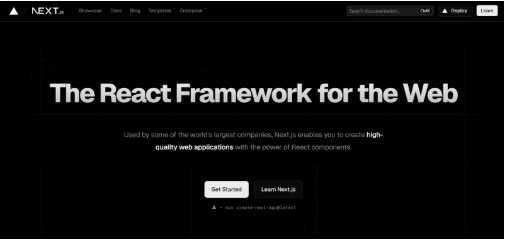
\includegraphics[width=0.7\textwidth]{root/react.png}
    \caption{NextJs}
\end{figure}
NextJS\cite{nextjs-docs} is a React framework for building high-quality, fast fullstack web applications. What sets it apart from plain React lies in its capabilities:

\begin{itemize}
\item Server-side Rendering (SSR) and Static Site Generation (SSG) optimize SEO and performance, which is difficult to achieve with vanilla React projects
\item App Router based on file system simplifies routing and application structure organization
\item Integrated API Routes enable building full-stack applications within a single project
\end{itemize}

These features make NextJS an ideal choice for modern web development, allowing developers to create high-performance, SEO-friendly applications without the complexities typically associated with setting up server-side rendering or API routes in standard React applications. The framework's file-based routing system also significantly reduces the boilerplate code needed for navigation and page structure, making development more efficient and maintainable.

The built-in optimization features and server-side capabilities of NextJS address many of the limitations of client-side React applications, particularly in areas of performance, SEO, and initial page load times. This makes it particularly valuable for production-grade applications that need to maintain high performance while scaling.
\subsection{CSS Framework - Tailwind CSS}
\begin{figure}[H]
    \centering
    
\includegraphics[width=0.8\textwidth]{root/tallwindcss.png}
    \caption{Tailwind CSS}
\end{figure}
TailwindCSS represents a utility-first approach to CSS, enabling rapid and consistent interface development. This framework provides a pre-defined utility classes system, along with a JIT (Just-In-Time) compiler that optimizes file size. The main advantages of TailwindCSS include rapid development speed, easy maintenance, and excellent scalability.

The recently introduced Tailwind v4 brings even more significant improvements \cite{tailwindcss-docs}. Performance has been dramatically enhanced, with build speeds up to 5 times faster than previous versions. The key enhancements include:

\begin{itemize}
\item Performance Optimization: Full builds in the new engine are up to 5x faster, and incremental builds are over 100x faster, measured in microseconds
\item Unified Toolchain: Built-in import handling, vendor prefixing, and syntax transforms, with no additional tooling required
\item CSS-first Configuration: A reimagined developer experience where you can customize and extend the framework directly in CSS instead of using a JavaScript configuration file
\item Modern Web Features: Built on native cascade layers, wide-gamut colors, and including first-class support for modern CSS features like container queries, @starting-style, popovers, and more
\end{itemize}

These improvements significantly enhance the development experience, making it easier and faster to build modern web applications while maintaining the framework's core principles of utility-first CSS. The shift to CSS-first configuration and improved build performance makes Tailwind v4 an even more powerful tool for web development.


\section{UI Library}  % Becomes "Appendix B: Second Appendix Title"
\subsection{Shadcn/ui}
\begin{figure}[H]
    \centering
    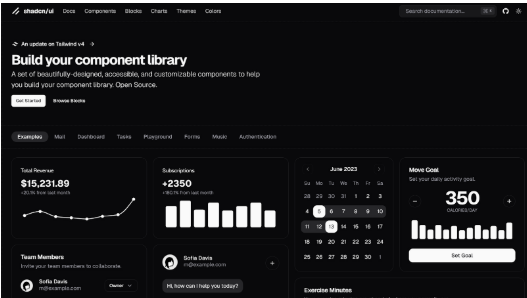
\includegraphics[width=0.8\textwidth]{root/shad.png}
    \caption{Tailwind CSS}
\end{figure}
Shadcn/ui \cite{shadcnui} is a component library featuring modern and aesthetically pleasing interfaces. At its core, Shadcn is built on RadixUI but has been modified to focus on accessibility and customization capabilities. The library is particularly suitable for projects requiring:

\begin{itemize}
\item Components with high accessibility standards and easy customization options
\item Complete source code control
\item Comprehensive TypeScript support
\end{itemize}

Additionally, Shadcn provides Blocks - pre-built code blocks for common functionalities such as Login forms, Dashboards, etc. These blocks come with various layout options and are ready to use, enabling developers to quickly implement them in their projects.

Key advantages of using Shadcn/ui include:

\begin{itemize}
\item High-quality, reusable components that maintain consistency across applications
\item A "copy-paste" approach that gives developers full control over the code
\item Strong integration with modern development tools and frameworks
\item Pre-built UI blocks that accelerate development of common features
\item Extensive styling options through Tailwind CSS integration
\end{itemize}

The library's focus on accessibility and customization, combined with its pre-built blocks, makes it an excellent choice for developers looking to build professional, user-friendly interfaces while maintaining development efficiency.
\subsection{React Flow ( XYFLow )}
\begin{figure}[H]
    \centering
    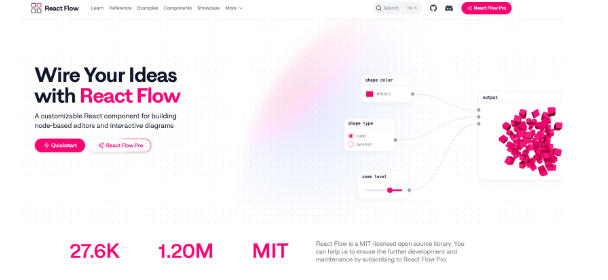
\includegraphics[width=0.8\textwidth]{figures/reactxy.png}
    \caption{React Flow}
\end{figure}
React Flow is a specialized library for building node-based interfaces. This library provides a simple yet powerful API for creating interactive diagrams, workflows, and node-based editors. React Flow stands out with its efficient handling of large graphs, support for custom nodes, and interactive features such as zoom, pan, and events handling.

Key features that make React Flow powerful \cite{reactflow}:

\begin{itemize}
\item Efficient rendering of complex node-based diagrams
\item Fully customizable nodes and edges
\item Comprehensive interaction capabilities
\item Seamless integration with React and TypeScript
\item Built-in support for common graph operations
\end{itemize}

\chapter{Project Architecture} 

These technology stacks combine to create a powerful ecosystem for modern web development. Each component serves a specific purpose:

\begin{itemize}
\item TypeScript ensures type safety and improved developer experience
\item Next.js provides a comprehensive framework for full-stack applications
\item TailwindCSS simplifies styling with its utility-first approach
\item Shadcn/ui delivers high-quality, accessible components
\item React Flow enables complex node-based interface development
\end{itemize}

Together, these technologies form a robust and popular stack that's particularly well-suited for enterprise projects requiring high maintainability and scalability. The integration between these tools creates a seamless development experience, allowing teams to build sophisticated web applications efficiently while maintaining code quality and performance.
\section{Root Directory}
\begin{figure}[H]
    \centering
    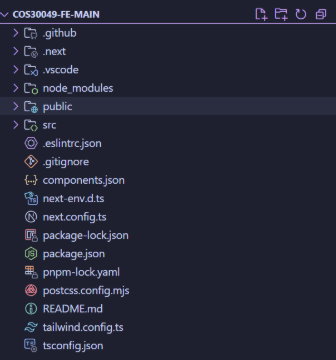
\includegraphics[width=0.55\textwidth]{figures/architecture.png}
    \caption{Architecture}
\end{figure}
Contains essential configuration files for the project:

\begin{itemize}
\item next.config.ts: Configuration for Next.js framework
\item tailwind.config.ts: Configuration for TailwindCSS
\item tsconfig.json: TypeScript configuration file
\item package.json: Manages project dependencies and scripts
\end{itemize}

These configuration files are crucial for setting up the development environment and maintaining consistency across the project.
\subsection{Public}
\begin{figure}[H]
    \centering
    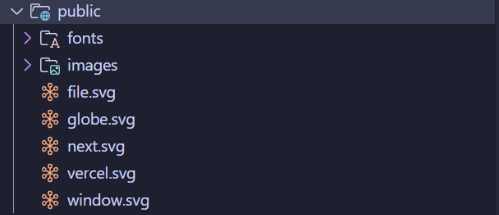
\includegraphics[width=0.6\textwidth, keepaspectratio]{figures/Public.png}
    \caption{Public}
\end{figure}
Manages static resources of the application:

\begin{itemize}
\item fonts: Typography fonts (Figtree, Poppins)
\item images: Images organized by modules
\item SVG assets and other resources
\end{itemize}
\subsection{Src}
\begin{figure}[H]
    \centering
    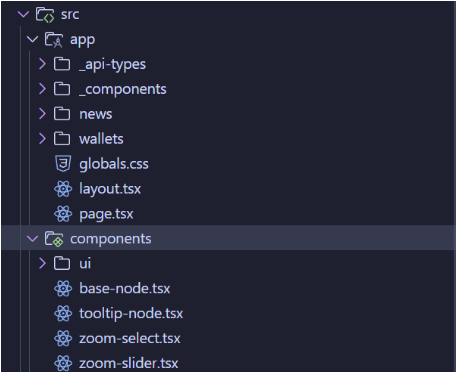
\includegraphics[width=0.55\textwidth]{figures/src.png}
    \caption{Src}
\end{figure}
Main directory containing application source code, organized into modules:

\begin{itemize}
\item app: Components and pages following Next.js App Router structure
    \begin{itemize}
    \item \_api-types: API type definitions
    \item \_components: Shared components for landing page
    \item news: News module
    \item wallets: Wallet management module, including details and transactions
    \end{itemize}
\item components: Reusable components
    \begin{itemize}
    \item ui: Basic components from Shadcn/ui
    \item Base components for common functions
    \end{itemize}
\item lib: Common utilities and types
    \begin{itemize}
    \item utils.ts: Utility functions
    \item types.ts: Shared type definitions
    \item typegen.ts: Automatic type generation tool
    \end{itemize}

\end{itemize}


\end{document}
